% ===================================================================
%  PRESENTACIÓN PROYECTO GLOBAL INTEGRADOR — AyME 2026
%  Calderón, Joaquín — Castel, Francisco
%  Compilar con: pdflatex main_presentacion.tex
% ===================================================================
\documentclass[aspectratio=169,t]{beamer}

% ---------- Paquetes ----------
\usepackage[utf8]{inputenc}
\usepackage[T1]{fontenc}
\usepackage{lmodern}                                  % evita 'T1/cmss/b/n undefined'
\usepackage[spanish]{babel}
\usepackage{amsmath,amssymb,amsfonts,bm,mathtools}
\usepackage{tikz}
\usepackage{graphicx}
\usepackage{xcolor}
\usepackage{booktabs}
\usepackage{array}
\usepackage{tabularx}
\usepackage{multirow}
\usepackage{textcomp}

% ---------- Tema minimalista (función > estética) ----------
\usetheme{default}
\setbeamertemplate{navigation symbols}{}    % sin barra de navegación

\definecolor{uncBlue}{RGB}{0,68,124}
\definecolor{uncGray}{RGB}{90,90,90}

\setbeamercolor{frametitle}{fg=uncBlue}
\setbeamerfont{frametitle}{series=\bfseries,size=\large}
\setbeamertemplate{frametitle}{%
  \vspace{2mm}\hspace{2mm}\insertframetitle\vspace{-2mm}%
}

% ---------- Footer azul con subsección a la izquierda y número a la derecha ----------
\setbeamercolor{footer_blue}{bg=uncBlue, fg=white}
\setbeamertemplate{footline}{%
  \leavevmode%
  \hbox{%
    \begin{beamercolorbox}[wd=\paperwidth, ht=2.8ex, dp=1.2ex, leftskip=3mm, rightskip=3mm]{footer_blue}%
      \scriptsize\insertsubsection\hfill\insertframenumber\,/\,\inserttotalframenumber%
    \end{beamercolorbox}%
  }%
}
\setbeamercolor{normal text}{fg=black}
\setbeamertemplate{itemize item}{\color{uncBlue}\textbullet}
\setbeamertemplate{itemize subitem}{\color{uncGray}--}
\setbeamercolor{definition box}{fg=black,bg=uncBlue!6}

\newcommand{\definitionbox}[2]{%
  \begin{beamercolorbox}[wd=\linewidth,sep=0.9ex,leftskip=0.9ex,rightskip=0.9ex]{definition box}%
    {\small\bfseries\color{uncBlue}#1}\par\vspace{0.2mm}%
    {\small #2}%
  \end{beamercolorbox}%
}

% ---------- Nombres centralizados de los bloques ----------
\newcommand{\SecPresentacion}{Presentación del problema}
\newcommand{\SecMecanico}{Subsistema mecánico equivalente}
\newcommand{\SecElectromagnetico}{Subsistema electromagnético en coordenadas qd0}
\newcommand{\SecTermico}{Subsistema térmico}
\newcommand{\SecNLGlobal}{Sistema No Lineal Global}
\newcommand{\SecLPV}{Linealización Jacobiana (LPV)}
\newcommand{\SecLTI}{Obtención del modelo LTI equivalente}
\newcommand{\SecAnalisisLTI}{Análisis del modelo LTI aumentado}
\newcommand{\SecDinamica}{Respuesta dinámica en dominio del tiempo}
\newcommand{\SecControlador}{Diseño y análisis del controlador en cascada}
\newcommand{\SecVerifSpecs}{Verificación de desempeño: Especificaciones de operación}
\newcommand{\SecVerifOffset}{Verificación de desempeño: Offset de estado estacionario}
\newcommand{\SecVerifNoIdealidades}{Verificación de desempeño: No idealidades y comportamiento térmico}
\newcommand{\SecDiscretizacion}{Discretización del controlador}
\newcommand{\SecSoftware}{Codificación del software de control}

% ---------- Macros para tipos de slide ----------

% Slide-figura: título de sección + imagen al máximo
%   \figslide{TÍTULO DE SECCIÓN}{nombre_imagen.png}{epigrafe (caption del informe)}
\newcommand{\figslide}[3]{%
  \begin{frame}{#1}
    \vspace{1.5mm}
    \centering
    \includegraphics[width=0.96\textwidth,height=0.70\textheight,keepaspectratio]{imagenes/#2}\par
    \vspace{1.5mm}
    {\scriptsize\textit{#3}}
  \end{frame}
}

% Slide-ecuación destacada
\newcommand{\eqslide}[2]{%
  \begin{frame}{#1}
    \vspace{0.8cm}
    #2
    \vfill
  \end{frame}
}

% Fila de agenda: el bloque activo se destaca y el resto queda atenuado.
\newcommand{\AgendaItem}[3]{%
  \ifnum#1=#2
    {\scriptsize\bfseries\color{uncBlue}%
      \hyperlink{sec:#1}{\makebox[2.2em][r]{#1.}\hspace{0.7em}%
      \parbox[t]{0.86\textwidth}{#3}}\par}%
  \else
    {\scriptsize\color{black!26}%
      \hyperlink{sec:#1}{\makebox[2.2em][r]{#1.}\hspace{0.7em}%
      \parbox[t]{0.86\textwidth}{#3}}\par}%
  \fi
  \vspace{0.35mm}%
}

% Contenido común de agenda.
\newcommand{\AgendaBody}[1]{%
    \vspace{3mm}
    {\Large\bfseries\color{uncBlue}Tabla de contenidos\par}
    \vspace{2mm}
    \begin{minipage}{0.94\textwidth}
      \AgendaItem{1}{#1}{\SecPresentacion}
      \AgendaItem{2}{#1}{\SecMecanico}
      \AgendaItem{3}{#1}{\SecElectromagnetico}
      \AgendaItem{4}{#1}{\SecTermico}
      \AgendaItem{5}{#1}\SecNLGlobal
      \AgendaItem{6}{#1}{\SecLPV}
      \AgendaItem{7}{#1}{\SecLTI}
      \AgendaItem{8}{#1}{\SecAnalisisLTI}
      \AgendaItem{9}{#1}{\SecDinamica}
      \AgendaItem{10}{#1}{\SecControlador}
      \AgendaItem{11}{#1}{\SecVerifSpecs}
      \AgendaItem{12}{#1}{\SecVerifOffset}
      \AgendaItem{13}{#1}{\SecVerifNoIdealidades}
      \AgendaItem{14}{#1}{\SecDiscretizacion}
      \AgendaItem{15}{#1}{\SecSoftware}
    \end{minipage}
    \vfill
}

% Diapositiva de agenda entre bloques internos.
\newcommand{\AgendaSlide}[1]{%
  \begin{frame}[plain]
    \AgendaBody{#1}
  \end{frame}
}

% Diapositiva de agenda que además define el destino navegable del bloque.
\newcommand{\AgendaSlideTarget}[2]{%
  \begin{frame}[plain]
    \hypertarget{#2}{}%
    \AgendaBody{#1}
  \end{frame}
}

% Arranque de bloque principal: actualiza navegación y emite la agenda.
\newcommand{\StartProjectSection}[2]{%
  \section{#2}%
  \subsection{#2}%
  \AgendaSlideTarget{#1}{sec:#1}%
}

% ---------- Metadatos ----------
\title{Proyecto Global Integrador}
\subtitle{Control de Accionamiento de CA con Motor Sincrónico de Imanes Permanentes (PMSM)}
\author{Joaquín Calderón \and Francisco Castel}
\institute{UNCuyo --- Facultad de Ingeniería --- Ingeniería Mecatrónica\\
Espacio Curricular 311: Automática y Máquinas Eléctricas}
\date{2026}

\begin{document}

% -------------------------------------------------------------------
%  SLIDE 1 — PORTADA
% -------------------------------------------------------------------
\begin{frame}[plain]
  \centering
  \vspace{4mm}
  {\small UNIVERSIDAD NACIONAL DE CUYO\\
  Facultad de Ingeniería --- Ingeniería Mecatrónica\par}

  \vspace{3mm}
  {\small\color{uncGray} Espacio Curricular 311 --- Automática y Máquinas Eléctricas\par}

  \vspace{5mm}
  \rule{0.85\textwidth}{1pt}

  \vspace{5mm}
  {\huge\bfseries\color{uncBlue} Proyecto Global Integrador\par}

  \vspace{3mm}
  {\Large Control de Accionamiento de CA con\\Motor Sincrónico de Imanes Permanentes\par}

  \vspace{4mm}
  \rule{0.85\textwidth}{1pt}

  \vspace{3mm}
  {\large \textbf{Alumnos:}\par}
  \vspace{1mm}
  {\normalsize Joaquín Calderón \quad (Leg.\ 13839) \quad --- \quad Francisco Castel \quad (Leg.\ 13784)\par}

  \vspace{3mm}
  {\normalsize Mendoza, Argentina --- 2026\par}
\end{frame}

% -------------------------------------------------------------------
%  SLIDE 2 — ALCANCE Y OBJETIVOS
% -------------------------------------------------------------------
\begin{frame}{Alcance y objetivos del proyecto}
  \vspace{4mm}

  \textbf{Objetivos:}
  \begin{itemize}
    \item Modelado matemático completo del accionamiento (NL, LPV y LTI equivalente).
    \item Análisis estructural (estabilidad, observabilidad, controlabilidad).
    \item Diseño de controlador en cascada (modulador de torque + PID externo + observador).
    \item Verificación de desempeño: especificaciones de operación, offset y no idealidades.
    \item Discretización del controlador y codificación del software de control.
  \end{itemize}

  \vspace{3mm}
  \textbf{Componentes del sistema físico:}
  \begin{itemize}
    \item Máquina PMSM trifásica.
    \item Inversor trifásico desde CC.
    \item Reductor planetario rígido.
    \item Brazo manipulador 1~GDL.
    \item Sensores: encoder en eje motor, 3 sensores de corriente de fase, RTD en bobinado.
  \end{itemize}
\end{frame}

% -------------------------------------------------------------------
%  SLIDE 3 — ÍNDICE / MAPA DEL TRABAJO
% -------------------------------------------------------------------
\begin{frame}{Mapa de la presentación}
  \vspace{3mm}

  \begin{columns}[T]
    \column{0.48\textwidth}
    \textbf{Modelado y análisis}
    \begin{enumerate}\scriptsize
      \item \SecPresentacion.
      \item \SecMecanico.
      \item \SecElectromagnetico.
      \item \SecTermico.
      \item \SecNLGlobal
      \item \SecLPV.
      \item \SecLTI.
      \item \SecAnalisisLTI.
    \end{enumerate}

    \column{0.48\textwidth}
    \textbf{Control y verificación}
    \begin{enumerate}\scriptsize\setcounter{enumi}{8}
      \item \SecDinamica.
      \item \SecControlador.
      \item \SecVerifSpecs.
      \item \SecVerifOffset.
      \item \SecVerifNoIdealidades.
      \item \SecDiscretizacion.
      \item \SecSoftware.
    \end{enumerate}
  \end{columns}
\end{frame}

% ===================================================================
%  BLOQUE B1 — PRESENTACIÓN DEL PROBLEMA
% ===================================================================

\StartProjectSection{1}{\SecPresentacion}
% -------------------------------------------------------------------
%  SLIDE 4 -- Presentación del problema
% -------------------------------------------------------------------

% -------------------------------------------------------------------
%  SLIDE 5 — Sistema bajo estudio (overview)
% -------------------------------------------------------------------
\figslide{Sistema bajo estudio, Subsistemas y variables medidas}{diagrama_completo.png}{Diagrama general del accionamiento con sus tres subsistemas (eléctrico, electromagnético-térmico, mecánico) y las variables medidas en cada uno.}

% -------------------------------------------------------------------
%  SLIDE 6 — Carga mecánica: brazo 1 GDL
% -------------------------------------------------------------------
\figslide{Carga mecánica: brazo manipulador rígido de 1 GDL}{brazo_1gdl.png}{Robot manipulador elemental de 1 g.d.l en plano vertical (péndulo rígido actuado).}

% -------------------------------------------------------------------
%  SLIDE 7 — Especificaciones físicas
% -------------------------------------------------------------------
\begin{frame}{Especificaciones físicas del sistema}
\vspace{2mm}

\renewcommand{\arraystretch}{1.05}
\footnotesize
\begin{columns}[T,onlytextwidth]

% --- Columna izquierda: Mecánica (10 filas) ---
\column{0.52\textwidth}
\centering
\resizebox{\linewidth}{!}{%
\begin{tabular}{|l|l|l|}
\hline
\multicolumn{3}{|c|}{\textbf{Mecánica (carga, transmisión y rotor)}} \\
\hline
\textbf{Símb.} & \textbf{Descripción} & \textbf{Valor} \\
\hline
$r$        & Relación de reducción         & $120{:}1$ \\
$g$        & Aceleración gravedad          & $9{,}80665$~m/s$^2$ \\
$m$        & Masa del brazo                & $1{,}0$~kg \\
$l_{cm}$   & Long.\ centro de masa         & $0{,}25$~m \\
$l_l$      & Longitud al extremo           & $0{,}50$~m \\
$m_l$      & Masa carga útil (variable)    & $0\dots 1{,}5$~kg \\
$b_l$      & Fricción articulación         & $0{,}1$~Nms/rad \\
$T_{ld}$   & Perturbación de contacto      & $0\pm 5$~N$\cdot$m \\
$J_m$      & Inercia rotor (m+caja)        & $14{\times}10^{-6}$~kg\,m$^2$ \\
$b_m$      & Fricción rotor (m+caja)       & $15{\times}10^{-6}$~Nms/rad \\
\hline
\end{tabular}%
}

% --- Columna derecha: Eléctrica (5 filas) + Térmico (5 filas vertical) ---
\column{0.46\textwidth}
\centering
\resizebox{\linewidth}{!}{%
\begin{tabular}{|l|l|l|}
\hline
\multicolumn{3}{|c|}{\textbf{Eléctrica (PMSM)}} \\
\hline
\textbf{Símb.} & \textbf{Descripción} & \textbf{Valor} \\
\hline
$P_p$         & Pares de polos              & $3$ \\
$\lambda'^r_m$  & Flujo de imanes             & $0{,}016$~Wb \\
$L_d$         & Inductancia eje directo     & $6{,}6$~mH \\
$L_q$         & Inductancia eje cuadratura  & $5{,}8$~mH \\
$L_{ls}$      & Inductancia dispersión      & $0{,}8$~mH \\
\hline
\end{tabular}%
}

\vspace{1.5mm}

\resizebox{\linewidth}{!}{%
\begin{tabular}{|l|l|l|}
\hline
\multicolumn{3}{|c|}{\textbf{Térmico}} \\
\hline
\textbf{Símb.} & \textbf{Descripción} & \textbf{Valor} \\
\hline
$R_{sREF}$            & $R_s$ @ $20\,^\circ$C            & $1{,}02$~$\Omega$ \\
$\alpha_{Cu}$         & Coef.\ térmico del cobre         & $3{,}9{\times}10^{-3}$~/$^\circ$C \\
$C_{ts}$              & Capacitancia térmica del estator & $0{,}818$~W/($^\circ$C/s) \\
$R_{ts\text{-}amb}$   & Resistencia térmica al ambiente  & $146{,}7$~$^\circ$C/W \\
$\tau_{ts\text{-}amb}$ & $R_{ts\text{-}amb}\cdot C_{ts}$ & $\approx 120$~s \\
\hline
\end{tabular}%
}

\end{columns}
\end{frame}

% -------------------------------------------------------------------
%  SLIDE 8 — Especificaciones operativas y límites
% -------------------------------------------------------------------
\begin{frame}{Especificaciones operativas y límites a respetar}
\vspace{2mm}
\centering
\renewcommand{\arraystretch}{1.2}
\resizebox{\textwidth}{!}{%
\footnotesize
\begin{tabular}{|l|l|c|l|}
\hline
\textbf{Componente} & \textbf{Magnitud} & \textbf{Valor} & \textbf{Observación} \\
\hline
\multirow{2}{*}{Caja reductora (salida)}
   & Velocidad nominal $n_{l,nom}$                       & $60$~rpm ($\omega_{l,nom}=6{,}28$~rad/s)       & Régimen continuo \\
   & Torque nominal/pico $T_{q,nom}\,/\,T_{q,max}$       & $17{,}0\,/\,45{,}0$~N$\cdot$m                  & Pico: aceleración corta \\
\hline
\multirow{4}{*}{Motor PMSM (estator)}
   & Velocidad nominal rotor $n_{m,nom}$                 & $6600$~rpm ($\omega_{m,nom}=691{,}15$~rad/s)   & $\to$ salida reductor $=6600/r=55$~rpm $<60$~rpm $\checkmark$ \\
   & Tensión nominal línea $V_{sl,nom}$                  & $30$~Vca rms                                   & $V_{sf,nom}=V_{sl,nom}/\sqrt{3}$ \\
   & Corriente nominal/pico $I_{s,nom}\,/\,I_{s,max}$    & $0{,}4\,/\,2{,}0$~Aca rms                      & Pico: corta duración \\
   & Temperatura máxima bobinado $T_{s,max}^\circ$       & $115$~\textdegree{}C                           & RTD de protección \\
\hline
\multirow{2}{*}{Inversor trifásico}
   & Tensión máxima línea $V_{sl,max}$                   & $48$~Vca rms                                   & Saturación dura \\
   & Frecuencia eléctrica $f_e$                          & $[-330,\,0,\,+330]$~Hz                         & Signo $\Rightarrow$ sentido de giro \\
\hline
\multirow{2}{*}{Perturbaciones externas}
   & Torque de contacto $T_{ld}$                         & $0\pm 5{,}0$~N$\cdot$m                         & Asumido escalón \\
   & Temperatura ambiente $T_{amb}^\circ$                & $[-15,\,+40]$~\textdegree{}C                    \\
\hline
\end{tabular}%
}
\end{frame}

% ===================================================================
%  BLOQUE B2 — SUBSISTEMA MECÁNICO EQUIVALENTE
% ===================================================================

\StartProjectSection{2}{\SecMecanico}
% -------------------------------------------------------------------
%  SLIDE 9 -- Subsistema mecánico equivalente
% -------------------------------------------------------------------

% -------------------------------------------------------------------
%  SLIDE 10 — Modelado de la carga mecánica
% -------------------------------------------------------------------
\begin{frame}{Modelado de la carga mecánica (péndulo 1 GDL)}
\vspace{3mm}

\textbf{Ecuación dinámica:}
\begin{equation*}
J_l\,\dot{\omega}_l(t) = T_q(t) - b_l\,\omega_l(t) - T_l(t)
\end{equation*}

\textbf{Torque de carga} $\rightarrow$ T.Perturbacion = T.gravitatorio + T.contacto:
\begin{equation*}
T_l(t) = g\,k_l\,\sin\!\big(\theta_l(t)\big) + T_{ld}(t)
\end{equation*}

\textbf{Parámetros equivalentes referidos al eje de salida del reductor:}
\begin{align*}
J_l &= m\,l_{cm}^2 + J_{cm} + m_l\,l_l^2 \;=\; 0{,}0833 + [0\dots 0{,}375]\;\;\text{kg}\cdot\text{m}^2 \\
k_l &= m\,l_{cm} + m_l\,l_l \;=\; 0{,}25 + [0\dots 0{,}75]\;\;\text{kg}\cdot\text{m}
\end{align*}

\vspace{1mm}
{\small Relación cinemática: $\dot{\theta}_l(t)=\omega_l(t)$.}
\end{frame}

% -------------------------------------------------------------------
%  SLIDE 11 — Tren de transmisión rígido
% -------------------------------------------------------------------
\begin{frame}{Tren de transmisión rígido}
\vspace{4mm}

\textbf{Hipótesis del modelo equivalente:}
\begin{itemize}
\item Ausencia de \textit{backlash} (juego mecánico nulo).
\item Ausencia de elasticidad torsional (acoplamiento rígido ideal).
\item Inercia y fricción internas ya incluidas en $J_m$ y $b_m$.
\end{itemize}

\vspace{4mm}
\textbf{Relaciones de transformación motor $\leftrightarrow$ carga:}
\begin{equation*}
\omega_l(t) = \frac{1}{r}\,\omega_m(t)
\qquad\qquad
T_q(t) = r\,T_d(t)
\qquad\qquad
\theta_l(t) = \frac{1}{r}\,\theta_m(t)
\end{equation*}

\vspace{4mm}
{\small La rigidez del tren permite tratar carga, transmisión y rotor como una única unidad mecánica de 1~GDL, simplificando el modelo a un único subsistema mecánico equivalente.}
\end{frame}

% -------------------------------------------------------------------
%  SLIDE 12 — Subsistema mecánico del rotor
% -------------------------------------------------------------------
\begin{frame}{Subsistema mecánico del rotor de la PMSM}
\vspace{4mm}

\textbf{Ecuación dinámica del rotor (balance de torques):}
\begin{equation*}
J_m\,\dot{\omega}_m(t) = T_m(t) - b_m\,\omega_m(t) - T_d(t)
\end{equation*}

\textbf{Cinemática del rotor:}
\begin{equation*}
\dot{\theta}_m(t) = \omega_m(t)
\end{equation*}

\textbf{Variables del balance:}
\begin{itemize}
\item $T_m(t)$: torque electromagnético entregado por las corrientes del estator vía la interacción con el flujo de los imanes (se deriva en la sección electromagnética: $T_m = \tfrac{3}{2}P_p\lambda'^r_m i_{qs}^r + \tfrac{3}{2}P_p(L_d-L_q)i_{ds}^r i_{qs}^r$).
\item $T_d(t)$: torque de reacción transferido al tren de transmisión, despejada en la combinación algebraica con el péndulo (slide siguiente).
\item $J_m,\,b_m$: parámetros nominales del conjunto rotor + caja.
\end{itemize}
\end{frame}

% -------------------------------------------------------------------
%  SLIDE 13 — Combinación algebraica
% -------------------------------------------------------------------
\begin{frame}{Combinación: derivación del modelo equivalente}
\vspace{2mm}

\textbf{Paso 1.} Sustituyendo $\omega_l = \omega_m/r$ y $T_q = r\,T_d$ en la ecuación del péndulo:
\begin{equation*}
\tfrac{J_l}{r}\,\dot{\omega}_m(t) = r\,T_d(t) - \tfrac{b_l}{r}\,\omega_m(t) - T_l(t)
\end{equation*}

\textbf{Paso 2.} Despejando $T_d$ y usando $T_l = g\,k_l\sin(\theta_m/r)+T_{ld}$:
\begin{equation*}
T_d(t) = \tfrac{J_l}{r^2}\,\dot{\omega}_m + \tfrac{b_l}{r^2}\,\omega_m + \tfrac{1}{r}\!\left[g\,k_l\,\sin\!\big(\tfrac{\theta_m}{r}\big) + T_{ld}(t)\right]
\end{equation*}

\textbf{Paso 3.} Reemplazando $T_d$ en la ecuación del rotor ($J_m\dot{\omega}_m=T_m-b_m\omega_m-T_d$) y agrupando términos en $\dot{\omega}_m$ y $\omega_m$ se obtiene la ecuación equivalente compactada (siguiente slide).
\end{frame}

% -------------------------------------------------------------------
%  SLIDE 14 — Modelo equivalente al eje del motor
% -------------------------------------------------------------------
\begin{frame}{Modelo mecánico equivalente al eje del motor}
\vspace{8mm}

\begin{equation*}
\boxed{\;\;
J_{eq}\,\dot{\omega}_m(t) = T_m(t) - b_{eq}\,\omega_m(t) - \tfrac{1}{r}\!\left[g\,k_l\,\sin\!\big(\tfrac{\theta_m(t)}{r}\big) + T_{ld}(t)\right]
\;\;}
\end{equation*}

\vspace{8mm}
\textbf{¿Por qué se puede compactar?}
\begin{itemize}
\item La rigidez del tren ($r=120{:}1$) permite reflejar $J_l$ y $b_l$ al eje del motor con factor $1/r^2$.
\item Al desaparecer $T_d$ el sistema mecánico se reduce de 2 EDOs a 1 (orden 2 con $\theta_m,\omega_m$).
\item La perturbación gravitatoria queda como término no lineal $\sin(\theta_m/r)$.
\end{itemize}
\end{frame}

% -------------------------------------------------------------------
%  SLIDE 15 — Parámetros equivalentes
% -------------------------------------------------------------------
\begin{frame}{Parámetros mecánicos equivalentes (valores nominales)}
\vspace{3mm}

\textbf{Definiciones:}
\begin{equation*}
J_{eq} = J_m + \frac{J_l}{r^2}
\qquad\qquad
b_{eq} = b_m + \frac{b_l}{r^2}
\end{equation*}

\vspace{4mm}
\textbf{Evaluación numérica con $r=120$:}\par
\vspace{2mm}
\centering
\renewcommand{\arraystretch}{1.25}
\begin{tabular}{|l|c|c|c|}
\hline
\textbf{Magnitud} & \textbf{Mínima ($m_l=0$)} & \textbf{Máxima ($m_l=1{,}5$)} & \textbf{Unidad} \\
\hline
$J_l$    & $0{,}0833$              & $0{,}4583$              & kg$\cdot$m$^2$ \\
$k_l$    & $0{,}25$                & $1{,}375$               & kg$\cdot$m \\
$J_{eq}$ & $1{,}98\times 10^{-5}$  & $4{,}58\times 10^{-5}$  & kg$\cdot$m$^2$ \\
$b_{eq}$ & $2{,}19\times 10^{-5}$  & $2{,}19\times 10^{-5}$  & Nms/rad \\
\hline
\end{tabular}

\vspace{3mm}
{\small La incertidumbre $b_l\pm 0{,}03$ aporta $\pm 2{,}08{\times}10^{-6}$~Nms/rad a $b_{eq}$ (~$\sim 10\%$).}
\end{frame}

% -------------------------------------------------------------------
%  SLIDE 16 — Ecuaciones de estado del subsistema mecánico
% -------------------------------------------------------------------
\begin{frame}{Ecuaciones de estado del subsistema mecánico}
\vspace{2mm}

\textbf{Forma escalar:}
\begin{equation*}
\begin{cases}
\dot{\theta}_m(t) = \omega_m(t) \\[4pt]
\dot{\omega}_m(t) = -\dfrac{b_{eq}}{J_{eq}}\,\omega_m(t) -\dfrac{g\,k_l}{J_{eq}\,r}\,\sin\!\big(\tfrac{\theta_m(t)}{r}\big) +\dfrac{1}{J_{eq}}\,T_m(t) -\dfrac{1}{J_{eq}\,r}\,T_{ld}(t) \\[6pt]
y(t) = \theta_m(t)
\end{cases}
\end{equation*}

\vspace{2mm}
\textbf{Forma matricial} --- el término $\sin(\cdot)$ impide escribir $\dot{\bm{x}}=\bm{A}\bm{x}+\bm{B}\bm{u}$ estándar; el sistema es \textbf{no lineal}:
\begin{equation*}
\begin{bmatrix}\dot{\theta}_m \\ \dot{\omega}_m\end{bmatrix} =
\underbrace{\begin{bmatrix}\omega_m \\[2pt] -\tfrac{g\,k_l}{J_{eq}\,r}\sin\!\big(\tfrac{\theta_m}{r}\big) -\tfrac{b_{eq}}{J_{eq}}\,\omega_m\end{bmatrix}}_{\bm{f}(\bm{x})}
+
\underbrace{\begin{bmatrix}0 & 0 \\[2pt] \tfrac{1}{J_{eq}} & -\tfrac{1}{J_{eq}\,r}\end{bmatrix}}_{\bm{B}}
\begin{bmatrix}T_m(t) \\ T_{ld}(t)\end{bmatrix}
\end{equation*}
\end{frame}

% ===================================================================
%  BLOQUE B3 — SUBSISTEMA ELECTROMAGNÉTICO QD0 + PARK
% ===================================================================

\StartProjectSection{3}{\SecElectromagnetico}
% -------------------------------------------------------------------
%  SLIDE 17 -- Subsistema electromagnético en coordenadas rotóricas $qd0$
% -------------------------------------------------------------------

% -------------------------------------------------------------------
%  SLIDE 18 — Marco de referencia rotórico (concepto y cinemática)
% -------------------------------------------------------------------
\begin{frame}{Marco de referencia rotórico ($qd0$)}
\vspace{3mm}

\textbf{Posición angular del rotor en coordenadas eléctricas:}
\begin{equation*}
\theta_r(t) \equiv P_p\,\theta_m(t)
\qquad\Longleftrightarrow\qquad
\omega_r(t) = P_p\,\omega_m(t)
\end{equation*}
\end{frame}

% -------------------------------------------------------------------
%  SLIDE 19 — Tensiones trifásicas en abc (entregadas por el inversor)
% -------------------------------------------------------------------
\begin{frame}{Tensiones trifásicas referidas al estator ($abc$)}
\vspace{4mm}

\textbf{Componentes de fase del estator:}
\begin{align*}
v_{as}(t) &\approx \sqrt{2}\,\tfrac{V_{sl}(t)}{\sqrt{3}}\,\cos\!\big(\theta_{ev}(t)\big) \\
v_{bs}(t) &\approx \sqrt{2}\,\tfrac{V_{sl}(t)}{\sqrt{3}}\,\cos\!\big(\theta_{ev}(t) - \tfrac{2\pi}{3}\big) \\
v_{cs}(t) &\approx \sqrt{2}\,\tfrac{V_{sl}(t)}{\sqrt{3}}\,\cos\!\big(\theta_{ev}(t) + \tfrac{2\pi}{3}\big)
\end{align*}

con $V_{sl}(t)$ el \textbf{módulo de la tensión de línea} (notación de la guía).


\textbf{Vector trifásico de tensiones del estator:}
\begin{equation*}
\bm{\mathrm{v}}_{abcs}(t) \equiv \big[\,v_{as}(t),\;v_{bs}(t),\;v_{cs}(t)\,\big]^T
\end{equation*}

\textbf{Frecuencia eléctrica del estator (variable manipulable por el inversor):}
\begin{equation*}
\omega_e(t) \equiv 2\pi f_e(t) = \frac{d\theta_{ev}(t)}{dt}
\qquad\text{con}\quad f_e\in[-330,\,0,\,+330]\;\text{Hz}
\end{equation*}

{\small El signo de $f_e$ define la secuencia $abc$/$acb$ y por ende el sentido de giro del campo rotante.}
\end{frame}

% -------------------------------------------------------------------
%  SLIDE 20 — Matriz de Park K_s
% -------------------------------------------------------------------
\begin{frame}{Transformación de Park: matriz $K_s(\theta_r)$}
\vspace{3mm}

\textbf{Relación directa $abc \rightarrow qd0$:}
\begin{equation*}
\bm{x}^{r}_{qd0s}(t) = K_s\!\big(\theta_r(t)\big)\;\bm{x}_{abcs}(t)
\qquad\text{con}\qquad \bm{x}\in\{\bm{v},\,\bm{i},\,\bm{\lambda}\}
\end{equation*}

\textbf{Matriz de Park (convención estándar de Krause):}
\begin{equation*}
K_s(\theta_r) = \frac{2}{3}
\begin{bmatrix}
\cos\theta_r & \cos\!\big(\theta_r-\tfrac{2\pi}{3}\big) & \cos\!\big(\theta_r+\tfrac{2\pi}{3}\big) \\[4pt]
\sin\theta_r & \sin\!\big(\theta_r-\tfrac{2\pi}{3}\big) & \sin\!\big(\theta_r+\tfrac{2\pi}{3}\big) \\[4pt]
\tfrac{1}{2} & \tfrac{1}{2} & \tfrac{1}{2}
\end{bmatrix}
\end{equation*}

\textbf{Transformación inversa $qd0\rightarrow abc$:}
\begin{equation*}
\bm{x}_{abcs}(t) = K_s^{-1}\!\big(\theta_r(t)\big)\;\bm{x}^{r}_{qd0s}(t)
\end{equation*}

{\small El factor $2/3$ se elige para que las amplitudes pico se preserven al transformar (convención \emph{amplitud-invariante}).}
\end{frame}

% -------------------------------------------------------------------
%  SLIDE 21 — Ecuaciones de tensión en qd0 (rotor)
% -------------------------------------------------------------------
\begin{frame}{Tensiones de estator referidas al rotor ($qd0$)}
\vspace{3mm}

\textbf{Eje cuadratura ($q$):}
\begin{equation*}
v^{r}_{qs}(t) = R_s\!\big(T_s^\circ\big)\,i^{r}_{qs}(t) + L_q\,\frac{d i^{r}_{qs}(t)}{dt} + \big[\,\lambda'^r_m + L_d\,i^{r}_{ds}(t)\,\big]\,\omega_r(t)
\end{equation*}

\textbf{Eje directo ($d$):}
\begin{equation*}
v^{r}_{ds}(t) = R_s\!\big(T_s^\circ\big)\,i^{r}_{ds}(t) + L_d\,\frac{d i^{r}_{ds}(t)}{dt} - L_q\,i^{r}_{qs}(t)\,\omega_r(t)
\end{equation*}

\textbf{Eje homopolar ($0$):}
\begin{equation*}
v^{r}_{0s}(t) = R_s\!\big(T_s^\circ\big)\,i^{r}_{0s}(t) + L_{ls}\,\frac{d i^{r}_{0s}(t)}{dt}
\end{equation*}

\vspace{1mm}
{\small \textbf{Estructura común:} caída resistiva + caída inductiva + acoplamiento de velocidad (FCEM de imanes y/o acoplamiento cruzado $qd$).}
\end{frame}

% -------------------------------------------------------------------
%  SLIDE 22 — Identificación de los acoplamientos
% -------------------------------------------------------------------
\begin{frame}{Identificación física de los acoplamientos}
\vspace{4mm}

\textbf{Eje $q$:}
\begin{equation*}
v^{r}_{qs} = \underbrace{R_s\,i^{r}_{qs}}_{\text{disipación}} + \underbrace{L_q\tfrac{di^{r}_{qs}}{dt}}_{\text{inductivo}} + \underbrace{\lambda'^r_m\,\omega_r}_{\text{FCEM de imanes}} + \underbrace{L_d\,i^{r}_{ds}\,\omega_r}_{\text{acopl.\ cruzado $d\to q$}}
\end{equation*}

\textbf{Eje $d$:}
\begin{equation*}
v^{r}_{ds} = \underbrace{R_s\,i^{r}_{ds}}_{\text{disipación}} + \underbrace{L_d\tfrac{di^{r}_{ds}}{dt}}_{\text{inductivo}} \underbrace{-\,L_q\,i^{r}_{qs}\,\omega_r}_{\text{acopl.\ cruzado $q\to d$}}
\end{equation*}

\vspace{2mm}
\textbf{Observaciones clave:}
\begin{itemize}\small
\item $R_s$ depende de la temperatura $T_s^\circ(t) \;\Rightarrow$ acoplamiento con el subsistema térmico.
\item Los términos $\propto \omega_r$ acoplan dinámicamente la dinámica eléctrica con la mecánica.
\item Si se impone $i^{r}_{ds}\equiv 0$ (\textbf{control vectorial con campo orientado}), el acoplamiento cruzado del eje $q$ se reduce a $\lambda'^r_m\omega_r$ y la dinámica de $i^{r}_{qs}$ se vuelve lineal de primer orden.
\end{itemize}
\end{frame}

% -------------------------------------------------------------------
%  SLIDE 23 — Torque electromagnético
% -------------------------------------------------------------------
\begin{frame}{Torque electromagnético: imanes + reluctancia}
\vspace{8mm}

\begin{equation*}
\boxed{\;\;
T_m(t) = \underbrace{\tfrac{3}{2}\,P_p\,\lambda'^r_m\,i^{r}_{qs}(t)}_{\text{torque de imanes}} \;+\; \underbrace{\tfrac{3}{2}\,P_p\,(L_d - L_q)\,i^{r}_{ds}(t)\,i^{r}_{qs}(t)}_{\text{torque de reluctancia}}
\;\;}
\end{equation*}

\vspace{8mm}
\textbf{Implicaciones para el control:}
\begin{itemize}\small
\item Con polos no salientes ideales ($L_d=L_q$): subsiste solo el torque por imanes, lineal en $i^{r}_{qs}$.
\item En esta máquina $L_d>L_q$ (rotor de polos ligeramente salientes), por lo que $i^{r}_{ds}\neq 0$ aporta torque de reluctancia.
\item \textbf{Estrategia base:} forzar $i^{r}_{ds}\equiv 0 \;\Rightarrow\; T_m = \tfrac{3}{2}P_p\lambda'^r_m\,i^{r}_{qs}$ (lineal y desacoplado).
\item \textbf{Estrategia extendida:} $i^{r}_{ds}\neq 0$ habilita \emph{field forcing} (refuerzo) y \emph{field weakening} (debilitamiento) — se analiza más adelante.
\end{itemize}
\end{frame}

% ===================================================================
%  BLOQUE B4 — TÉRMICO + MODELO NL GLOBAL + IRRELEVANCIA i_0s
% ===================================================================

\StartProjectSection{4}{\SecTermico}
%----
% -------------------------------------------------------------------
%  SLIDE 24 -- Subsistema térmico
% -------------------------------------------------------------------
%----
% -------------------------------------------------------------------
%  SLIDE 25 — Subsistema térmico: hipótesis del modelo
% -------------------------------------------------------------------
\begin{frame}{Subsistema térmico}
\vspace{6mm}

\textbf{Modelo simplificado equivalente de primer orden}, considerando:
\begin{itemize}
\item Solo \textbf{pérdidas eléctricas resistivas} por efecto Joule (calor) en el bobinado de estator.
\item Se \textbf{desprecian} las \textbf{pérdidas magnéticas} en el núcleo.
\item Transferencia de calor al ambiente solo por \textbf{conducción} y \textbf{convección natural}.
\item \textbf{Sin ventilación forzada}.
\end{itemize}
\end{frame}

% -------------------------------------------------------------------
%  SLIDE 26 — Subsistema térmico: estructura y dependencias
% -------------------------------------------------------------------
\begin{frame}{Dependencias}
\vspace{4mm}

\textbf{Dependencia de la resistencia con la temperatura} (modelo lineal del cobre):
\begin{equation*}
R_s\!\big(T_s^\circ(t)\big) = R_{sREF}\!\left[\,1 + \alpha_{Cu}\!\big(T_s^\circ(t) - T_{sREF}^\circ\big)\,\right]
\qquad T_{sREF}^\circ = 20\,^\circ\text{C}
\end{equation*}

\textbf{Pérdidas Joule en el bobinado} (potencia disipada por las corrientes en $qd0$):
\begin{equation*}
P_{s,perd}(t) = \tfrac{3}{2}\,R_s\!\big(T_s^\circ(t)\big)\;\big(\,i_{qs}^{r\,2}(t) + i_{ds}^{r\,2}(t) + 2\,i_{0s}^{r\,2}(t)\,\big)
\end{equation*}

\vspace{2mm}
{\small \textbf{Acoplamiento bidireccional con el subsistema eléctrico:} la temperatura modifica $R_s$, y a su vez $R_s$ determina las pérdidas Joule. Este lazo es una de las no linealidades del modelo global.}
\end{frame}

% -------------------------------------------------------------------
%  SLIDE 27 — Balance térmico y ecuación de estado
% -------------------------------------------------------------------
\begin{frame}{Balance térmico y ecuación de estado}
\vspace{3mm}

\textbf{Balance de potencia térmica:}
\begin{equation*}
C_{ts}\,\frac{dT_s^\circ(t)}{dt} = \underbrace{P_{s,perd}(t)}_{\text{generación}} \;-\; \underbrace{\frac{T_s^\circ(t) - T_{amb}^\circ(t)}{R_{ts\text{-}amb}}}_{\text{disipación al ambiente}}
\end{equation*}

\textbf{Ecuación de estado del subsistema térmico} (despejando $dT_s^\circ/dt$):
\begin{equation*}
\frac{dT_s^\circ(t)}{dt} = \frac{1}{C_{ts}}\!\left[\,\tfrac{3}{2}\,R_s\!\big(T_s^\circ\big)\big(i_{qs}^{r\,2}+i_{ds}^{r\,2}+2\,i_{0s}^{r\,2}\big) \;-\; \frac{T_s^\circ - T_{amb}^\circ}{R_{ts\text{-}amb}}\,\right]
\end{equation*}

\end{frame}
\StartProjectSection{5}{\SecNLGlobal}

% -------------------------------------------------------------------
%  SLIDE 28 — Modelo NL global: estados, entradas y salidas
% -------------------------------------------------------------------
\begin{frame}{Modelo NL global: estados, entradas y salidas}
\vspace{4mm}

\textbf{Vector de estado interno} (6 estados):
\begin{equation*}
\bm{x}_{NL}(t) = \big[\,\theta_m,\;\omega_m,\;i_{qs}^{r},\;i_{ds}^{r},\;i_{0s},\;T_s^\circ\,\big]^T
\end{equation*}

\textbf{Vector de entradas} (manipuladas + perturbaciónes):
\begin{equation*}
\bm{u}_{NL}(t) = \underbrace{\big[\,v_{qs}^{r},\;v_{ds}^{r},\;v_{0s}\,\big]^T}_{\text{manipuladas (vía Park del inversor)}} \;\;\cup\;\; \underbrace{\big[\,T_{ld},\;T_{amb}^\circ,\ g\,\big]^T}_{\text{perturbaciónes externas}}
\end{equation*}

\textbf{Variables observables y controladas:}
\begin{itemize}\small
\item \textbf{Medidas directamente:} $\theta_m$ (encoder), $\bm{i}_{abcs}$ (3 CT), $T_s^\circ$ (RTD).
\item \textbf{Controlada (no medida directamente):} $q(t)\equiv\theta_l(t) = \theta_m(t)/r$.
\end{itemize}
\end{frame}

% -------------------------------------------------------------------
%  SLIDE 29 — Modelo NL global: sistema de 6 EDOs
% -------------------------------------------------------------------
\begin{frame}{Modelo NL global: sistema de 6 EDOs acopladas}
\vspace{2mm}

\footnotesize
\begin{equation*}
\left\{
\begin{aligned}
\dot{\theta}_m &= \omega_m \\[1pt]
\dot{\omega}_m &= -\tfrac{b_{eq}}{J_{eq}}\omega_m - \tfrac{g\,k_l}{J_{eq}\,r}\sin\!\big(\tfrac{\theta_m}{r}\big) + \tfrac{1}{J_{eq}}\,T_m - \tfrac{1}{J_{eq}\,r}\,T_{ld} \\[1pt]
\dot{i}_{qs}^{r} &= \tfrac{1}{L_q}\!\left[\,v_{qs}^{r} - R_s\!\big(T_s^\circ\big)\, i_{qs}^{r} - \big(\lambda'^r_m + L_d\,i_{ds}^{r}\big)\,\omega_r\,\right] \\[1pt]
\dot{i}_{ds}^{r} &= \tfrac{1}{L_d}\!\left[\,v_{ds}^{r} - R_s\!\big(T_s^\circ\big)\, i_{ds}^{r} + L_q\,i_{qs}^{r}\,\omega_r\,\right] \\[1pt]
\dot{i}_{0s} &= \tfrac{1}{L_{ls}}\!\left[\,v_{0s} - R_s\!\big(T_s^\circ\big)\, i_{0s}\,\right] \\[1pt]
\dot{T}_s^\circ &= \tfrac{1}{C_{ts}}\!\left[\,\tfrac{3}{2}R_s\!\big(T_s^\circ\big)\big(i_{qs}^{r\,2}+i_{ds}^{r\,2}+2\,i_{0s}^{r\,2}\big) - \tfrac{T_s^\circ - T_{amb}^\circ}{R_{ts\text{-}amb}}\,\right]
\end{aligned}\right.
\end{equation*}
\normalsize

\vspace{1mm}
{\small \textbf{Con} $T_m = \tfrac{3}{2}P_p\lambda'^r_m\,i_{qs}^{r} + \tfrac{3}{2}P_p(L_d-L_q)\,i_{ds}^{r}\,i_{qs}^{r}$ \;y\; $\omega_r = P_p\omega_m$.\quad \textbf{No linealidades:} (i) gravitatoria $\sin(\theta_m/r)$; (ii) producto $i_{ds}^{r}\!\cdot\! i_{qs}^{r}$ en $T_m$; (iii) cuadráticas en $P_{s,perd}$; (iv) $R_s(T_s^\circ)$.}
\end{frame}

% -------------------------------------------------------------------
%  SLIDE 30 — Irrelevancia de la secuencia cero (neutro flotante)
% -------------------------------------------------------------------
\begin{frame}{Irrelevancia de la secuencia cero (caso general, neutro flotante)}
\vspace{4mm}

\textbf{Ley de Corrientes de Kirchhoff en el nodo neutro $n$:}
\begin{equation*}
i_a(t) + i_b(t) + i_c(t) \equiv 0
\qquad (\text{sin conductor externo de retorno})
\end{equation*}

\textbf{Consecuencia inmediata sobre la componente homopolar:}
\begin{equation*}
i_{0s}(t) = \tfrac{1}{3}\big(i_a + i_b + i_c\big) \equiv 0
\qquad\Longrightarrow\qquad
\boxed{\;i_{0s}(t) \equiv 0\;}
\end{equation*}

\textbf{Implicación sobre la ecuación de tensión del eje $0$:}
\begin{equation*}
v_{0s}(t) = R_s\!\big(T_s^\circ\big)\cdot 0 + L_{ls}\,\frac{d(0)}{dt} = 0
\end{equation*}

{\small \textbf{Conclusión:} bajo la hipótesis de caso geneal con neutro flotante, la ecuación de secuencia cero queda satisfecha de forma trivial y no contribuye a la dinámica del sistema.}
\end{frame}

% -------------------------------------------------------------------
%  SLIDE 31 — Modelo NL global reducido a 5 estados
% -------------------------------------------------------------------
\begin{frame}{Modelo NL global reducido a 5 estados}
\vspace{2mm}

\textbf{Estado reducido} y \textbf{entradas reducidas}:
\begin{equation*}
\bm{x}_{NL}(t) = \big[\,\theta_m,\;\omega_m,\;i_{qs}^{r},\;i_{ds}^{r},\;T_s^\circ\,\big]^T
\qquad
\bm{u}_{NL}(t) = \big[\,v_{qs}^{r},\;v_{ds}^{r},\;T_{ld},\;T_{amb}^\circ\,\big]^T
\end{equation*}

\textbf{Sistema dinámico (5 EDOs):}
\footnotesize
\begin{equation*}
\left\{
\begin{aligned}
\dot{\theta}_m &= \omega_m \\
\dot{\omega}_m &= -\tfrac{b_{eq}}{J_{eq}}\omega_m - \tfrac{g\,k_l}{J_{eq}\,r}\sin\!\big(\tfrac{\theta_m}{r}\big) + \tfrac{1}{J_{eq}}\,T_m(i_{qs}^{r},\,i_{ds}^{r}) - \tfrac{1}{J_{eq}\,r}\,T_{ld} \\
\dot{i}_{qs}^{r} &= \tfrac{1}{L_q}\!\big[\,v_{qs}^{r} - R_s\!\big(T_s^\circ\big)\, i_{qs}^{r} - (\lambda'^r_m + L_d\,i_{ds}^{r})\,\omega_r\,\big] \\
\dot{i}_{ds}^{r} &= \tfrac{1}{L_d}\!\big[\,v_{ds}^{r} - R_s\!\big(T_s^\circ\big)\, i_{ds}^{r} + L_q\,i_{qs}^{r}\,\omega_r\,\big] \\
\dot{T}_s^\circ &= \tfrac{1}{C_{ts}}\!\big[\,\tfrac{3}{2}R_s\!\big(T_s^\circ\big)(i_{qs}^{r\,2}+i_{ds}^{r\,2}) - \tfrac{T_s^\circ - T_{amb}^\circ}{R_{ts\text{-}amb}}\,\big]
\end{aligned}\right.
\end{equation*}
\normalsize

\vspace{1mm}
{\small Este modelo es la \textbf{planta de referencia} para los procesos de linealización (Jacobiana LPV) y de retroalimentación NL (LTI equivalente).}
\end{frame}

\subsection{Validación a lazo abierto del modelo no lineal}

% -------------------------------------------------------------------
%  SLIDE 32 - Diagrama Simulink completo (apertura de validación)
% -------------------------------------------------------------------
\figslide{Arquitectura de simulación a lazo abierto}{simulink_diagrama_completo.png}{Diagrama de bloques implementado en Simulink. Se destaca la estructura de validación con Transformaciones directa e inversa y la interconexión de los subsistemas.}

% -------------------------------------------------------------------
%  SLIDE 33 -- Ensayo a lazo abierto: respuesta electromecánica
% -------------------------------------------------------------------
\begin{frame}{Ensayo a lazo abierto: respuesta electromecánica}
\vspace{2mm}

\centering
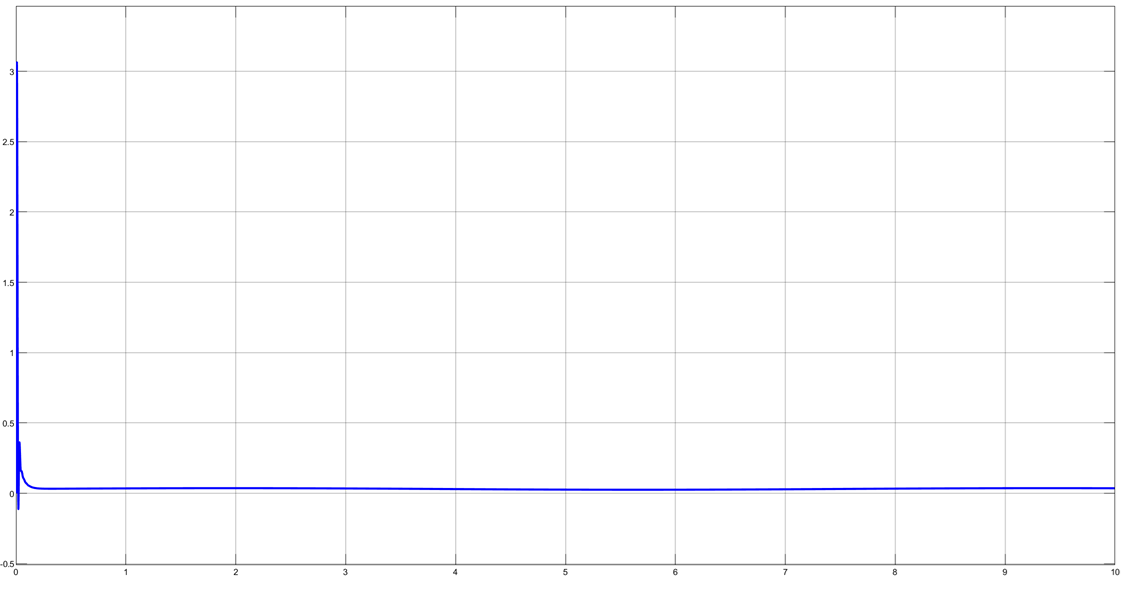
\includegraphics[width=0.82\textwidth,height=0.32\textheight,keepaspectratio]{imagenes/resultado_corriente.png}\par
{\scriptsize\textit{Respuesta dinámica al escalón $v_q=5$~V: corriente de estator $i_q$~[A] con transitorio inductivo y efecto de la FCEM.}}\par
\vspace{0.5mm}
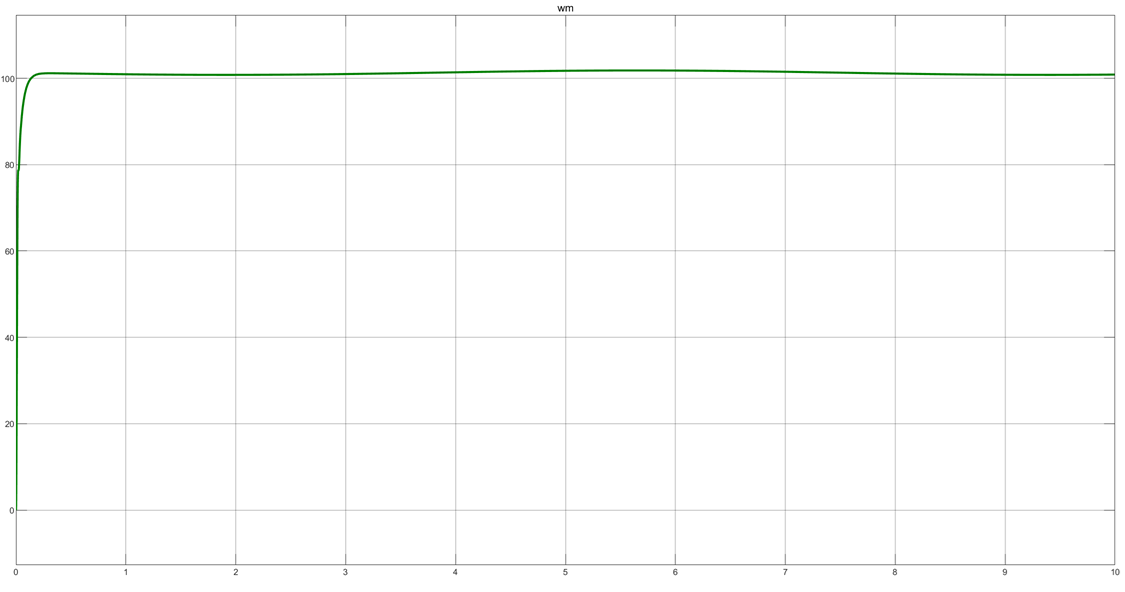
\includegraphics[width=0.82\textwidth,height=0.32\textheight,keepaspectratio]{imagenes/resultado_velocidad.png}\par
{\scriptsize\textit{Respuesta dinámica al escalón $v_q=5$~V: velocidad mecánica del rotor $\omega_m$~[rad/s].}}
\end{frame}

% -------------------------------------------------------------------
%  SLIDE 34 -- Ensayo a lazo abierto: respuesta térmica
% -------------------------------------------------------------------
\begin{frame}{Ensayo a lazo abierto: respuesta térmica}
\vspace{2mm}

\centering
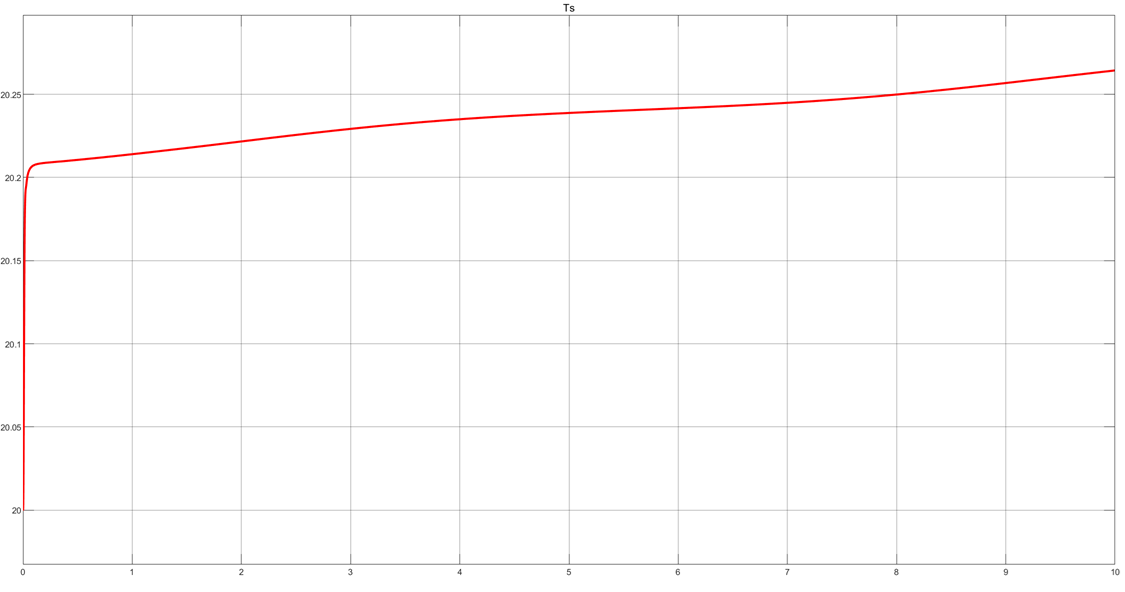
\includegraphics[width=0.86\textwidth,height=0.50\textheight,keepaspectratio]{imagenes/resultado_temperatura.png}\par
{\scriptsize\textit{Evolución de la temperatura del estator $T_s$. Nótese el cambio de pendiente provocado por la variación de la corriente durante el arranque.}}

\vspace{1mm}
\begin{itemize}\small
  \item Parte en $T_s(0)=20\,^\circ$C; calentamiento por pérdidas Joule.
  \item Pendiente mayor al arranque (corriente máxima, FCEM baja).
  \item Al crecer $\omega_m$ y caer $i_q$, baja la tasa de calentamiento.
\end{itemize}
\end{frame}

\StartProjectSection{6}{\SecLPV}
% -------------------------------------------------------------------
%  SLIDE 35 -- Linealización por Parámetros Variables - LPV
% -------------------------------------------------------------------

% -------------------------------------------------------------------
%  SLIDE 36 - Idea de linealización Jacobiana
% -------------------------------------------------------------------
\begin{frame}{Método de pequeñas señales: idea central}
\vspace{3mm}

\textbf{Descomposición en equilibrio + perturbación:}
\begin{equation*}
\bm{x}(t)=\bm{x}_O+\Delta\bm{x}(t),
\qquad
\bm{u}(t)=\bm{u}_O+\Delta\bm{u}(t)
\end{equation*}

\textbf{Modelo no lineal de partida:}
\begin{equation*}
\dot{\bm{x}}=\bm{f}(\bm{x},\bm{u})
\end{equation*}

\textbf{Taylor de primer orden en $(\bm{x}_O,\bm{u}_O)$:}
\begin{equation*}
\Delta\dot{\bm{x}}(t)\approx
\underbrace{\left.\frac{\partial \bm{f}}{\partial \bm{x}}\right|_O}_{\bm{A}_O}
\Delta\bm{x}(t)+
\underbrace{\left.\frac{\partial \bm{f}}{\partial \bm{u}}\right|_O}_{\bm{B}_O}
\Delta\bm{u}(t)
\end{equation*}

{\small Resultado: un modelo \textbf{lineal local} válido para pequeñas variaciones respecto del equilibrio elegido.}
\end{frame}

% -------------------------------------------------------------------
%  SLIDE 37 - Punto de operación
% -------------------------------------------------------------------
\begin{frame}{Punto de operación cuasiestático}
\vspace{3mm}

\textbf{Condiciones clave del equilibrio:}
\begin{itemize}
  \item \textbf{Cinemática:} $\dot{\theta}_{m,o}=\omega_{m,o}$ con $\omega_{m,o}$ constante.
  \item \textbf{Mecánica:} el torque electromagnético compensa fricción, gravedad y carga:
  \[
  0=-b_{eq}\omega_{m,o}+T_{m,o}-g\,k_l\sin\!\big(\theta_{m,o}/r\big)-T_{ld,o}/r
  \]
  \item \textbf{Eléctrica:} las corrientes $i^r_{qs,o}$, $i^r_{ds,o}$ quedan fijadas por las tensiones de equilibrio $v^r_{qs,o}$, $v^r_{ds,o}$.
  \item \textbf{Térmica:} la disipación Joule iguala al intercambio con ambiente:
  \[
  0=\tfrac{3}{2}R_s(T_{s,o}^\circ)\!\left(i^{r\,2}_{qs,o}+i^{r\,2}_{ds,o}\right)-\frac{T_{s,o}^\circ-T_{amb,o}^\circ}{R_{ts\text{-}amb}}
  \]
\end{itemize}

{\small Cada elección de $(\theta_{m,o},\omega_{m,o},i^r_{qs,o},i^r_{ds,o},T_{s,o}^\circ)$ define un \textbf{modelo local distinto}.}
\end{frame}

% -------------------------------------------------------------------
%  SLIDE 38 - Modelo incremental LPV
% -------------------------------------------------------------------
\begin{frame}{Modelo incremental LPV}
\vspace{3mm}

\textbf{Estado incremental reducido:}
\begin{equation*}
\Delta\bm{x}(t)=
\big[\,\Delta\theta_m,\;\Delta\omega_m,\;\Delta i_{qs}^{r},\;\Delta i_{ds}^{r},\;\Delta T_s^\circ\,\big]^T
\end{equation*}

\textbf{Entradas incrementales:}
\begin{equation*}
\Delta\bm{u}(t)=
\big[\,\Delta v_{qs}^{r},\;\Delta v_{ds}^{r},\;\Delta T_{ld},\;\Delta T_{amb}^\circ\,\big]^T
\end{equation*}

\textbf{Forma estructural:}
\begin{equation*}
\Delta\dot{\bm{x}}(t)=\bm{A}_O(\rho)\,\Delta\bm{x}(t)+\bm{B}_O(\rho)\,\Delta\bm{u}(t)
\end{equation*}

\textbf{Parámetros de operación} $\rho$:
\begin{equation*}
\rho=\big(\theta_{m,o},\;\omega_{m,o},\;i^r_{qs,o},\;i^r_{ds,o},i_{0s,o},\;T_{s,o}^\circ\big)
\end{equation*}

{\small En otras palabras: la dinámica es lineal para perturbaciónes pequeñas, pero \textbf{sus coeficientes cambian con el régimen de trabajo}.}
\end{frame}

% -------------------------------------------------------------------
%  SLIDE 39 (nueva) — Matriz Jacobiana A_0 completa + Gamma_th
% -------------------------------------------------------------------
\begin{frame}{Matriz Jacobiana $\bm{A}_O$ del modelo LPV}
\vspace{2mm}

\centering
\resizebox{\textwidth}{!}{$
\bm{A}_O = \begin{bmatrix}
0 & 1 & 0 & 0 & 0 & 0 \\[2pt]
-\dfrac{g\,k_l\cos\!\big(\theta_{m,o}/r\big)}{J_{eq}\,r^2} & -\dfrac{b_{eq}}{J_{eq}} & \dfrac{3 P_p\!\left[\lambda'^r_m + (L_d{-}L_q)\,i^r_{ds,o}\right]}{2\,J_{eq}} & \dfrac{3 P_p (L_d{-}L_q)\,i^r_{qs,o}}{2\,J_{eq}} & 0 & 0 \\[6pt]
0 & -\dfrac{P_p\!\left[\lambda'^r_m + L_d\,i^r_{ds,o}\right]}{L_q} & -\dfrac{R_{s,o}}{L_q} & -\dfrac{L_d P_p\,\omega_{m,o}}{L_q} & 0 & -\dfrac{R_{sREF}\,\alpha_{Cu}\,i^r_{qs,o}}{L_q} \\[6pt]
0 & \dfrac{L_q P_p\,i^r_{qs,o}}{L_d} & \dfrac{L_q P_p\,\omega_{m,o}}{L_d} & -\dfrac{R_{s,o}}{L_d} & 0 & -\dfrac{R_{sREF}\,\alpha_{Cu}\,i^r_{ds,o}}{L_d} \\[6pt]
0 & 0 & 0 & 0 & -\dfrac{R_{s,o}}{L_{ls}} & -\dfrac{R_{sREF}\,\alpha_{Cu}\,i_{0s,o}}{L_{ls}} \\[6pt]
0 & 0 & \dfrac{3 R_{s,o}\,i^r_{qs,o}}{C_{ts}} & \dfrac{3 R_{s,o}\,i^r_{ds,o}}{C_{ts}} & \dfrac{6 R_{s,o}\,i_{0s,o}}{C_{ts}} & \Gamma_{th}
\end{bmatrix}
$}

\vspace{1mm}
\textbf{Constante de disipación térmica acoplada} (elemento $A_{66}$):
\[
\Gamma_{th} = -\dfrac{1}{C_{ts}}\left[\dfrac{1}{R_{ts\text{-}amb}} - \dfrac{3\,R_{sREF}\,\alpha_{Cu}}{2}\!\left(2\,i_{0s,o}^{2} + i^{r\,2}_{ds,o} + i^{r\,2}_{qs,o}\right)\right]
\]
\end{frame}

% -------------------------------------------------------------------
%  SLIDE 40 (nueva) — Matrices de entrada B_o^c, B_o^d y modelo LPV global
% -------------------------------------------------------------------
\begin{frame}{Matrices de entrada y modelo LPV global}
\vspace{3mm}

\textbf{Matrices de entrada:}
\[
\bm{B}_o^c = \begin{bmatrix}
0 & 0 & 0 \\ 0 & 0 & 0 \\ \tfrac{1}{L_q} & 0 & 0 \\ 0 & \tfrac{1}{L_d} & 0 \\ 0 & 0 & \tfrac{1}{L_{ls}} \\ 0 & 0 & 0
\end{bmatrix}
\qquad\qquad
\bm{B}_o^d = \begin{bmatrix}
0 & 0 \\ -\tfrac{1}{J_{eq}\,r} & 0 \\ 0 & 0 \\ 0 & 0 \\ 0 & 0 \\ 0 & \tfrac{1}{C_{ts}\,R_{ts\text{-}amb}}
\end{bmatrix}
\]

\vspace{3mm}
\textbf{Modelo LPV global en forma matricial:}
\footnotesize
\[
\Delta\dot{\bm{x}}(t) = \bm{A}_O\,\Delta\bm{x}(t) \;+\; \bm{B}_o^c\!\begin{bmatrix}\Delta v_{qs}^{r}\\ \Delta v_{ds}^{r}\\ \Delta v_{0s}\end{bmatrix} \;+\; \bm{B}_o^d\!\begin{bmatrix}\Delta T_{ld}\\ \Delta T_{amb}^\circ\end{bmatrix}
\]
\normalsize
\end{frame}

\StartProjectSection{7}{\SecLTI}
% -------------------------------------------------------------------
%  SLIDE 41 -- Linealización por realimentación de no linealidades - Modelo LTI
% -------------------------------------------------------------------

% -------------------------------------------------------------------
%  SLIDE 41 - Ley mínima eje d
% -------------------------------------------------------------------
\begin{frame}{Segunda linealización: realimentación de no linealidades}
\vspace{3mm}

\textbf{Hipótesis de desacoplamiento:}
\begin{equation*}
i_{ds}^{r}(t)\equiv 0
\end{equation*}

\textbf{Ecuación original del eje $d$:}
\begin{equation*}
\dot{i}_{ds}^{r}(t)=\frac{1}{L_d}\Big[\,v_{ds}^{r}(t)-R_{s0}i_{ds}^{r}(t)+L_q\,i_{qs}^{r}(t)\,\omega_r(t)\Big]
\end{equation*}

\textbf{Ley de control mínima} para cancelar el acoplamiento cruzado:
\begin{equation*}
\boxed{\;v_{ds}^{r}(t)=-L_q\,i_{qs}^{r}(t)\,\omega_r(t)\;}
\end{equation*}

\textbf{Efecto físico buscado:}
\begin{itemize}
  \item forzar $i_{ds}^{r}\to 0$,
  \item orientar el flujo sobre el eje de imanes,
  \item dejar el torque proporcional solo a $i_{qs}^{r}$.
\end{itemize}
\end{frame}

% -------------------------------------------------------------------
%  SLIDE 42 - Modelo LTI nominal
% -------------------------------------------------------------------
\begin{frame}{Modelo LTI nominal resultante}
\vspace{2mm}

\textbf{Perturbación mecánica externa:} el torque de carga $T_l(t)$ se trata como entrada exógena del modelo.

\footnotesize
\begin{equation*}
\left\{
\begin{aligned}
\dot{\theta}_m &= \omega_m \\[2pt]
\dot{\omega}_m &= \frac{1}{J_{eq}}\!\left[\frac{3}{2}P_p\lambda'^r_m\,i_{qs}^r-b_{eq}\omega_m-\frac{1}{r}T_l\right] \\[4pt]
\dot{i}_{qs}^r &= \frac{1}{L_q}\!\left[-P_p\lambda'^r_m\,\omega_m-R_{s0}i_{qs}^r+v_{qs}\right]
\end{aligned}
\right.
\end{equation*}
\normalsize

\textbf{Estado nominal:}
\begin{equation*}
\bm{x}_{LTI}(t)=\big[\,\theta_m,\;\omega_m,\;i_{qs}^r\,\big]^T
\end{equation*}

{\small El torque de carga $T_l(t)$ se trata como entrada de perturbación externa (exógena), por lo que la matriz $\bm{A}$ resulta lineal e invariante en el tiempo.}
\end{frame}

% -------------------------------------------------------------------
%  SLIDE 43 - Forma matricial e interpretación
% -------------------------------------------------------------------
\begin{frame}{Forma matricial e interpretación física}
\vspace{2mm}

\centering
\resizebox{0.85\textwidth}{!}{$
\dot{\bm{x}}_{LTI}=
\underbrace{\begin{bmatrix}
0 & 1 & 0\\
0 & -\frac{b_{eq}}{J_{eq}} & \frac{3P_p\lambda'^r_m}{2J_{eq}}\\
0 & -\frac{P_p\lambda'^r_m}{L_q} & -\frac{R_{s0}}{L_q}
\end{bmatrix}}_{\bm{A}}
\bm{x}_{LTI}+
\underbrace{\begin{bmatrix}0\\0\\ \frac{1}{L_q}\end{bmatrix}}_{\bm{B}_c}v_{qs}
+
\underbrace{\begin{bmatrix}0\\-\frac{1}{rJ_{eq}}\\0\end{bmatrix}}_{\bm{B}_d}T_l
$}

\textbf{Interpretación del modelo:}
\begin{itemize}
  \item $\bm{A}$ contiene la planta electromecánica nominal.
  \item $\bm{B}_c$ muestra que la acción de control entra solo por el canal de corriente $q$.
  \item $\bm{B}_d$ inyecta la perturbación mecánica externa $T_l(t)$ (torque de carga).
\end{itemize}

{\small Esta separación es la base para el análisis posterior de estabilidad, funciones de transferencia y desempeño del controlador.}
\end{frame}

% -------------------------------------------------------------------
%  SLIDE 44 - Diagrama del LTI nominal
% -------------------------------------------------------------------
\figslide{Diagrama del modelo LTI nominal}{LTI equivalente_nominal.png}{Diagrama de bloques de estado del modelo LTI equivalente nominal.}

\subsection{Modelo LTI aumentado e implementación}
% -------------------------------------------------------------------
%  SLIDE 45 -- Modelo LTI aumentado e implementación
% -------------------------------------------------------------------

% -------------------------------------------------------------------
%  SLIDE 46 - Dinámica residual
% -------------------------------------------------------------------
\begin{frame}{Dinámica residual del eje $d$}
\vspace{3mm}

\textbf{Con la ley mínima} $v_{ds}^{r}=-L_q i_{qs}^{r}\omega_r$:
\begin{equation*}
\dot{i}_{ds}^{r}(t)= -\frac{R_{s0}}{L_d}\,i_{ds}^{r}(t)
\end{equation*}

\textbf{Solución temporal:}
\begin{equation*}
i_{ds}^{r}(t)=i_{ds}^{r}(0)\,e^{-\frac{R_{s0}}{L_d}t}
\end{equation*}

\textbf{Interpretación física:}
\begin{itemize}
  \item $i_{ds}^{r}$ no diverge ni excita modos adicionales acoplados.
  \item Decae exponencialmente hacia cero con constante de tiempo
  \[
  \tau_d=\frac{L_d}{R_{s0}}
  \]
  \item Esa dinámica residual es transitoria, pero conviene incorporarla al modelo para cubrir el caso general $i_{ds}^r(0)\neq 0$.
\end{itemize}
\end{frame}

% -------------------------------------------------------------------
%  SLIDE 47 - Ley complementaria eje q
% -------------------------------------------------------------------
\begin{frame}{Ley complementaria en el eje $q$}
\vspace{3mm}

\textbf{Acoplamiento residual sobre el eje $q$:}
\begin{equation*}
v_{qs}^{r}(t)=L_q\dot{i}_{qs}^{r}(t)+R_s i_{qs}^{r}(t)+\lambda'^r_m\omega_r(t)+
\underbrace{\omega_r(t)L_d i_{ds}^{r}(t)}_{\text{acoplamiento cruzado}}
\end{equation*}

\textbf{Ley de control complementaria:}
\begin{equation*}
\boxed{\;v_{qs}^{r*}(t)=v_{qs}(t)+\omega_r(t)L_d i_{ds}^{r}(t)\;}
\end{equation*}

\textbf{Resultado buscado:}
\begin{itemize}
  \item cancelar el término cruzado restante,
  \item conservar $v_{qs}(t)$ como nueva entrada lineal de control,
  \item obtener un modelo equivalente válido también para $i_{ds}^{r}(0)\neq 0$.
\end{itemize}
\end{frame}

% -------------------------------------------------------------------
%  SLIDE 48 - Modelo LTI aumentado escalar
% -------------------------------------------------------------------
\begin{frame}{Modelo LTI aumentado de cuarto orden}
\vspace{2mm}

\textbf{Estado aumentado:}
\begin{equation*}
\bm{x}_{aug}(t)=\big[\,\theta_m,\;\omega_m,\;i_{qs}^r,\;i_{ds}^{r}\,\big]^T
\end{equation*}

\footnotesize
\begin{equation*}
\left\{
\begin{aligned}
\dot{\theta}_m &= \omega_m \\[2pt]
\dot{\omega}_m &= \frac{1}{J_{eq}}\!\left[\frac{3}{2}P_p\lambda'^r_m\,i_{qs}^r-b_{eq}\omega_m-\frac{1}{r}T_l\right] \\[4pt]
\dot{i}_{qs}^r &= \frac{1}{L_q}\!\left[-P_p\lambda'^r_m\,\omega_m-R_{s0}i_{qs}^r+v_{qs}\right] \\[4pt]
\dot{i}_{ds}^{r} &= -\frac{R_{s0}}{L_d}\,i_{ds}^{r}
\end{aligned}
\right.
\end{equation*}
\normalsize

{\small La temperatura puede seguir simulándose aparte, pero la dinámica electromecánica lineal equivalente queda contenida en estos cuatro estados.}
\end{frame}

% -------------------------------------------------------------------
%  SLIDE 49 - Forma matricial aumentado
% -------------------------------------------------------------------
\begin{frame}{Forma matricial del modelo aumentado}
\vspace{2mm}

\centering
\resizebox{\textwidth}{!}{$
\dot{\bm{x}}_{aug}=
\underbrace{\begin{bmatrix}
0 & 1 & 0 & 0\\
0 & -\frac{b_{eq}}{J_{eq}} & \frac{3P_p\lambda'^r_m}{2J_{eq}} & 0\\
0 & -\frac{P_p\lambda'^r_m}{L_q} & -\frac{R_{s0}}{L_q} & 0\\
0 & 0 & 0 & -\frac{R_{s0}}{L_d}
\end{bmatrix}}_{\bm{A}_{aug}}
\bm{x}_{aug}+
\underbrace{\begin{bmatrix}0\\0\\ \frac{1}{L_q}\\0\end{bmatrix}}_{\bm{B}_c}v_{qs}
+
\underbrace{\begin{bmatrix}0\\-\frac{1}{rJ_{eq}}\\0\\0\end{bmatrix}}_{\bm{B}_d}T_l
$}

\textbf{Interpretación del modelo:}
\begin{itemize}
  \item el cuarto estado no realimenta a la dinámica nominal,
  \item pero queda explícitamente representado para cubrir condiciones iniciales no nulas,
  \item así el modelo sigue siendo útil para análisis y simulación comparativa.
\end{itemize}
\end{frame}

% -------------------------------------------------------------------
%  SLIDE 50 - Diagrama aumentado
% -------------------------------------------------------------------
\figslide{Diagrama del modelo LTI aumentado}{LTI equivalente_aumentado.png}{Diagrama de bloques de estado del modelo LTI equivalente aumentado.}

% -------------------------------------------------------------------
%  SLIDE 51 - Implementación sobre la planta NL
% -------------------------------------------------------------------
\figslide{Implementación sobre la planta no lineal}{NL con realimentacion NL.png}{Diagrama de bloques de implementación de la realimentación sobre la planta no lineal.}

% -------------------------------------------------------------------
%  SLIDE 53 - Comparación conceptual
% -------------------------------------------------------------------
\begin{frame}{LPV vs. LTI aumentado: comparación conceptual}
\vspace{2mm}

\centering
\footnotesize
\renewcommand{\arraystretch}{1.25}
\resizebox{\textwidth}{!}{%
\begin{tabular}{|>{\bfseries}p{0.18\textwidth}|p{0.41\textwidth}|p{0.41\textwidth}|}
\hline
\multicolumn{1}{|c|}{\color{uncBlue}\textbf{Aspecto}} &
\multicolumn{1}{c|}{\color{uncBlue}\textbf{LPV (pequeñas señales)}} &
\multicolumn{1}{c|}{\color{uncBlue}\textbf{LTI aumentado (realim.\ NL)}} \\
\hline\hline
Naturaleza de la linealización &
Expansión en Taylor truncada a 1\textsuperscript{er} orden (\emph{pequeña señal}). Sólo válida cerca de $(x_0,u_0)$. &
Algebraicamente exacto, sin Taylor. Cancela las NL inyectando tensiones virtuales calculadas dinámicamente. \\
\hline
Carga gravitacional (NL mecánica) &
Linealiza $\sin(\theta_{m0}/r)\to$ rigidez local. Aparece $A_{2,1}\propto\cos(\theta_{m0}/r)$: los polos mecánicos \textbf{cambian con la posición} del brazo. &
El torque de carga $T_l(t)$ ingresa como perturbación externa (exógena); no se deriva respecto de la posición, por lo que $A_{2,1}=0$ permanece \textbf{invariante}. \\
\hline
Subsistema térmico &
Conserva la influencia: $R_{s0}$ depende del equilibrio térmico $T_{s0}$ del Jacobiano. &
\textbf{Desacople térmico completo}: $R_s$ se trata como constante rígida en el transitorio rápido. \\
\hline
Estructura al forzar $I^r_{ds,o}\equiv 0$ &
Caso particular: el acoplamiento cruzado se vuelve puramente $\lambda'^r_m$ (sin reluctancia), coincidiendo con $A_{3,2}$ del LTI. &
\textbf{Es} el caso ideal de un LPV operando perpetuamente en $I^r_{ds,o}=0$, con el torque de carga $T_l(t)$ tratado como perturbación externa. \\
\hline
\end{tabular}%
}

\vspace{2mm}
{\scriptsize \textbf{Conclusión:} ambos modelos son comparables pero no equivalentes en su origen. El LTI aumentado puede interpretarse como el caso ideal del LPV con $I^r_{ds,o}\equiv 0$ y la gravedad tratada como entrada exógena.}
\end{frame}

\subsection{Variaciones de corriente en eje d}
% -----------------------------------------------------------

% -------------------------------------------------------------------
%  SLIDE 55 - ids como parametro
% -------------------------------------------------------------------
\begin{frame}{Corriente de eje $d$ como parámetro}
\vspace{3mm}

\textbf{Torque electromagnético en operación estacionaria:}
\begin{equation*}
T_m=\frac{3}{2}P_p\Big[\lambda'^r_m+(L_d-L_q)I^r_{ds,o}\Big]I^r_{qs,o}
\end{equation*}

\textbf{Qué cambia respecto del caso base:}
\begin{itemize}
  \item Con $I^r_{ds,o}=0$, el torque queda asociado al flujo de los imanes y a $I^r_{qs,o}$.
  \item Con $I^r_{ds,o}\neq 0$, aparece el aporte de reluctancia por saliencia.
  \item El mismo parámetro desplaza los autovalores del Jacobiano LPV.
\end{itemize}

{\small Esta es una lectura local del LPV: no reemplaza al LTI aumentado, sino que muestra cómo cambia el modelo alrededor de otros puntos de operación.}
\end{frame}

% -------------------------------------------------------------------
%  SLIDE 56 - Reforzamiento y debilitamiento
% -------------------------------------------------------------------
\figslide{Reforzamiento y debilitamiento de campo}{polosaliente_cilindrico.png}{Diagrama representativo de un rotor genérico de (c)(d)polos no salientes (arriba) y un (a)(b)rotor de polos salientes (abajo).}

% -------------------------------------------------------------------
%  SLIDE 57 - Migración con ids
% -------------------------------------------------------------------
% \begin{frame}{Migración dinámica con $I^r_{ds,o}$}
% {\small\color{uncGray}Barrido de los autovalores del Jacobiano LPV ante variación de $I^r_{ds,o}$, manteniendo el resto del punto de operación nominal. Se reproducen las dos tablas presentadas en el informe (sección 5.1.2.d).}\par
% \vspace{2mm}

% \centering
% \scriptsize
% \textbf{Debilitamiento de campo ($I^r_{ds,o}<0$)}\par\vspace{1mm}
% \begin{tabular}{|c|c|c|c|c|}
% \hline
% $I^r_{ds,o}$ [A] & $\lambda_1$ & $\lambda_2$ & $\lambda_{3,4}$ & $\lambda_5$ \\
% \hline
% $-1{,}2$ & $-1275{,}00$ & $-141{,}30$ & $-94{,}74 \pm j\,23{,}38$ & $-0{,}2657$ \\
% $-1{,}0$ & $-1275{,}00$ & $-145{,}62$ & $-92{,}61 \pm j\,47{,}75$ & $-0{,}2261$ \\
% $-0{,}8$ & $-1275{,}00$ & $-147{,}64$ & $-91{,}62 \pm j\,62{,}75$ & $-0{,}1963$ \\
% $-0{,}6$ & $-1275{,}00$ & $-148{,}88$ & $-91{,}01 \pm j\,74{,}74$ & $-0{,}1731$ \\
% $-0{,}4$ & $-1275{,}00$ & $-149{,}74$ & $-90{,}59 \pm j\,85{,}10$ & $-0{,}1544$ \\
% \hline
% \end{tabular}

% \vspace{2mm}
% \textbf{Reforzamiento de campo ($I^r_{ds,o}>0$)}\par\vspace{1mm}
% \begin{tabular}{|c|c|c|c|c|}
% \hline
% $I^r_{ds,o}$ [A] & $\lambda_1$ & $\lambda_2$ & $\lambda_{3,4}$ & $\lambda_5$ \\
% \hline
% $+0{,}2$ & $-1275{,}00$ & $-151{,}25$ & $-89{,}85 \pm j\,111{,}05$ & $-0{,}1157$ \\
% $+0{,}4$ & $-1275{,}00$ & $-151{,}57$ & $-89{,}70 \pm j\,118{,}65$ & $-0{,}1066$ \\
% $+0{,}6$ & $-1275{,}00$ & $-151{,}83$ & $-89{,}57 \pm j\,125{,}90$ & $-0{,}0986$ \\
% $+0{,}8$ & $-1275{,}00$ & $-152{,}05$ & $-89{,}46 \pm j\,132{,}85$ & $-0{,}0917$ \\
% $+1{,}0$ & $-1275{,}00$ & $-152{,}24$ & $-89{,}37 \pm j\,139{,}56$ & $-0{,}0857$ \\
% \hline
% \end{tabular}
% \normalsize

% \vspace{1mm}
% \raggedright
% {\scriptsize \textbf{Conclusiones del barrido:}
% (i) la parte imaginaria de $\lambda_{3,4}$ crece monotónicamente con $I^r_{ds,o}$ $\Rightarrow$ aumenta $\omega_n$ electromecánica;
% (ii) la parte real de $\lambda_{3,4}$ se mantiene en torno a $-91$~rad/s $\Rightarrow$ el amortiguamiento absoluto no se degrada;
% (iii) $\lambda_1$ (eléctrico rápido) y los modos restantes permanecen invariantes o varían levemente.}
% \end{frame}

% -------------------------------------------------------------------
%  SLIDE 58 - Mapa migración de polos LPV con I_ds (parte 1)
% -------------------------------------------------------------------
\figslide{Mapa de migración de polos con $I^r_{ds,o}$ --- vista global}{migracion_ids_1.png}{Mapa de migración de polos del modelo LPV al variar $I^r_{ds,o}$: vista global del plano $s$.}

% -------------------------------------------------------------------
%  SLIDE 59 - Mapa migración de polos LPV con I_ds (parte 2 - zoom)
% -------------------------------------------------------------------
\figslide{Mapa de migración de polos con $I^r_{ds,o}$ --- zoom}{migracion_ids_2.png}{Mapa de migración de polos del modelo LPV al variar $I^r_{ds,o}$: zoom sobre los polos electromecánicos.}


\subsection{Funciones de Transferencia}

\StartProjectSection{8}{\SecAnalisisLTI}
% -------------------------------------------------------------------
%  SLIDE 60 - Planteo de funciones de transferencia
% -------------------------------------------------------------------
\begin{frame}{Funciones de transferencia del LTI aumentado}
\vspace{3mm}

\textbf{Condiciones usadas para obtenerlas:}
\begin{itemize}
  \item Modelo incremental con $\bm{x}_{aug}(0)=\bm{0}$.
  \item Resistencia constante: $R_s=R_{s0}$.
  \item El torque de carga $T_l(t)$ se trata como perturbación externa: no aparece ningún término no lineal en la matriz $\bm{A}_{aug}$.
  \item Como $i_{ds}^{r}$ queda desacoplado, la relación entrada-salida se obtiene con el subsistema nominal de tercer orden.
\end{itemize}

\begin{equation*}
G(s)=\bm{C}\,(s\bm{I}-\bm{A})^{-1}\bm{B}
\end{equation*}
\end{frame}

% -------------------------------------------------------------------
%  SLIDE 61 - Funciones de transferencia finales
% -------------------------------------------------------------------
\begin{frame}{Funciones de transferencia obtenidas}
\vspace{2mm}

\small
\begin{equation*}
\Delta_3(s)=
s^3+
\left(\frac{b_{eq}}{J_{eq}}+\frac{R_{s0}}{L_q}\right)s^2+
\left(\frac{b_{eq}R_{s0}}{J_{eq}L_q}+
\frac{3P_p^2{\lambda'^r_m}^{\,2}}{2J_{eq}L_q}\right)s
\end{equation*}

\vspace{2mm}
\resizebox{\textwidth}{!}{$
G_1(s)=\frac{\theta_m(s)}{v_{qs}(s)}
=
\frac{\dfrac{3P_p\lambda'^r_m}{2J_{eq}L_q}}{\Delta_3(s)}
\qquad\qquad
G_2(s)=\frac{\theta_m(s)}{T_l(s)}
=
\frac{-\dfrac{1}{rJ_{eq}}\left(s+\dfrac{R_{s0}}{L_q}\right)}{\Delta_3(s)}
$}
\normalsize


\end{frame}



% -------------------------------------------------------------------
%  SLIDE 62 - Estabilidad a lazo abierto
% -------------------------------------------------------------------
\begin{frame}{Autovalores y estabilidad a lazo abierto}
\vspace{1mm}

\definitionbox{Estabilidad interna}{Un sistema lineal es estable si, ante condiciones iniciales finitas y sin entradas externas, sus estados permanecen acotados. Si además todos los modos libres decaen a cero, el sistema es asintóticamente estable.}
\vspace{1mm}

{\small
\begin{equation*}
\det(s\bm{I}-\bm{A}_{aug})=
\underbrace{\left(s+\frac{R_{s0}}{L_d}\right)}_{\lambda_4}
\underbrace{s}_{\lambda_1}
\underbrace{\left(s^2+a_2s+a_1\right)}_{\lambda_{2,3}}
\end{equation*}
}

\footnotesize
\textbf{Valores nominales:}
\begin{itemize}\setlength{\itemsep}{0pt}
  \item $\lambda_1=0$: integrador cinemático de posición ($\theta_m$ como cuasi variable de estado).
  \item $\lambda_{2,3}=-91{,}7\pm j\,148{,}0$: modo electromecánico subamortiguado, $\zeta\simeq0{,}527$.
  \item $\lambda_4=-160{,}3$: dinámica residual de $i_{ds}^{r}$, con $\tau_d\simeq6{,}24$ ms.
\end{itemize}

\textbf{Conclusión:} el subsistema físico ($\omega_m$, $i_{qs}^r$, $i_{ds}^{r}$) es \textbf{estable}. El polo en el origen no es un modo energético: $\theta_m$ es una \textbf{cuasi variable de estado} (coordenada acumulada, no almacena energía) incorporada para formular el control de posición; su deriva en lazo abierto no implica pérdida de estabilidad.
\end{frame}

% -------------------------------------------------------------------
%  SLIDE 63 - Mapa polos y ceros
% -------------------------------------------------------------------
\figslide{Mapa de polos y ceros a lazo abierto}{polos_ceros_LA.png}{Mapa de polos (cuadrados sólidos) y ceros (círculos vacíos) a lazo abierto para ambas funciones de transferencia del modelo LTI aumentado. El polo cancelado de $i_{ds}^r$ se indica con rombo rojo.}

\subsection{Variaciones paramétricas}
% -------------------------------------------------------------------
%  SLIDE 64 — Variaciones paramétricas
% -------------------------------------------------------------------

% -------------------------------------------------------------------
%  SLIDE 65 - Variacion de Rs
% -------------------------------------------------------------------
\figslide{Migración ante variación de $R_s$}{migracion_Rs.png}{Migración de polos y ceros en el plano $s$ (izq.) y variación de $\omega_n$ y $\zeta$ (der.) ante cambios en $R_s$.}

% -------------------------------------------------------------------
%  SLIDE 66 - Variacion de carga
% -------------------------------------------------------------------
\figslide{Migración ante variación de carga}{migracion_ml.png}{Migración de polos ante variación de masa de carga $m_l$ (izq.) y variación de $\omega_n$ y $\zeta$ (der.).}


\subsection{Observabilidad y Controlabilidad}
% -------------------------------------------------------------------
%  SLIDE 64 — Observabilidad y Controlabilidad
% -------------------------------------------------------------------
% -------------------------------------------------------------------
%  SLIDE 67 — Propiedades del modelo aumentado
% -------------------------------------------------------------------
\begin{frame}{Observabilidad y Controlabilidad}
\vspace{2mm}
\begin{columns}[T,onlytextwidth]

\begin{column}{0.49\textwidth}
\definitionbox{Observabilidad}{
$\bm{x}^\star\neq\bm{0}$ es no observable si:
\[
\bm{y}(t)=\bm{C}e^{\bm{A}t}\bm{x}^\star=\bm{0},\quad \forall t\geq0
\]

}
\vspace{2mm}
\begin{itemize}
  \item ¿Puede reconstruirse $\bm{x}_{aug}$ midiendo solo $\theta_m$ o solo $\omega_m$?
\end{itemize}
\end{column}

\begin{column}{0.49\textwidth}
\definitionbox{Controlabilidad}{
Existe $\bm{u}(t)$ en $[0,T]$ tal que:
\[
\bm{x}(0)=\bm{x}_0,\qquad \bm{x}(T)=\bm{0}
\]

}

\vspace{2mm}
\begin{itemize}
  \item ¿Puede actuarse sobre todos los estados usando solo $v_{qs}$?
\end{itemize}
\end{column}

\end{columns}

\end{frame}

% -------------------------------------------------------------------
%  SLIDE 68 - Observabilidad desde theta
% -------------------------------------------------------------------
\begin{frame}{Observabilidad desde posición}
\vspace{3mm}

\begin{equation*}
\mathcal{O}_\theta=
\begin{bmatrix}
\bm{C}_\theta\\
\bm{C}_\theta\bm{A}\\
\bm{C}_\theta\bm{A}^2\\
\bm{C}_\theta\bm{A}^3
\end{bmatrix},
\qquad
\operatorname{rango}(\mathcal{O}_\theta)=3<4
\end{equation*}

\textbf{Resultado:}
\begin{itemize}
  \item $\theta_m$ se mide directamente.
  \item $\omega_m$ aparece como derivada de $\theta_m$.
  \item $i_{qs}^r$ se manifiesta por el acoplamiento electromecánico.
  \item $i_{ds}^{r}$ no aparece: no acopla con la salida.
\end{itemize}
\end{frame}

% -------------------------------------------------------------------
%  SLIDE 69 - Observabilidad desde velocidad
% -------------------------------------------------------------------
\begin{frame}{Observabilidad desde velocidad}
\vspace{3mm}

\begin{equation*}
\mathcal{O}_\omega=
\begin{bmatrix}
\bm{C}_\omega\\
\bm{C}_\omega\bm{A}\\
\bm{C}_\omega\bm{A}^2\\
\bm{C}_\omega\bm{A}^3
\end{bmatrix},
\qquad
\operatorname{rango}(\mathcal{O}_\omega)=2<4
\end{equation*}

\textbf{Estados no observables:}
\begin{itemize}
  \item $\theta_m$: la velocidad no contiene la condición inicial de posición.
  \item $i_{ds}^{r}$: sigue siendo un modo interno desacoplado.
\end{itemize}

\vspace{3mm}
{\small \textbf{Conclusión:} No se requiere un sensor de velocidad, simplemente con un sensor de posición es posible estimar la velocidad.}
\end{frame}

% -------------------------------------------------------------------
%  SLIDE 70 - Controlabilidad desde vqs
% -------------------------------------------------------------------
\begin{frame}{Controlabilidad desde $v_{qs}$}
\vspace{3mm}

\begin{equation*}
\mathcal{C}_{v_q}=
\begin{bmatrix}
\bm{B}_c & \bm{A}\bm{B}_c & \bm{A}^2\bm{B}_c & \bm{A}^3\bm{B}_c
\end{bmatrix},
\qquad
\operatorname{rango}(\mathcal{C}_{v_q})=3<4
\end{equation*}

\textbf{Estado no controlable desde $v_{qs}$:}
\begin{itemize}
  \item $i_{ds}^{r}$, porque la cuarta fila queda desacoplada y $B_c(4)=0$.
\end{itemize}
\end{frame}

% -------------------------------------------------------------------
%  SLIDE 71 - Entrada adicional vds
% -------------------------------------------------------------------
\begin{frame}{Entrada adicional en eje $d$}
\vspace{2mm}

\begin{equation*}
\bm{B}_{ext}=
\begin{bmatrix}
0 & 0\\
0 & 0\\
\frac{1}{L_q} & 0\\
0 & \frac{1}{L_d}
\end{bmatrix},
\qquad
\operatorname{rango}(\mathcal{C}_{ext})=4
\end{equation*}

\textbf{Interpretación:}
\begin{itemize}
  \item Matemáticamente, $v_{ds}^{r}$ completa la controlabilidad del modelo aumentado.
  \item En la estrategia adoptada, esa tensión ya se usa por la ley mínima para forzar $i_{ds}^{r}\to0$.
  \item No se trata de un grado de libertad libre para el control externo de posición.
\end{itemize}
\end{frame}

% ===================================================================
%  BLOQUE — Simulación Dinámica
%  (señales, Simulink, theta_m, omega_m, i_qs con errores)
% ===================================================================

\StartProjectSection{9}{\SecDinamica}
\subsection{Simulación dinámica NL vs LTI aumentado}
% -------------------------------------------------------------------
%  SLIDE 73 -- Simulación Dinámica: Modelo NL vs LTI Aumentado
% -------------------------------------------------------------------

% -------------------------------------------------------------------
%  SLIDE 74 — Planteo de la simulación
% -------------------------------------------------------------------
\begin{frame}{Planteo de la simulación}
\vspace{4mm}

\textbf{Condiciones del ensayo:}
\begin{itemize}
\item Tres condiciones iniciales: $i_{ds}^{r}(0) \in \{\,0,\;+0{,}5,\;-0{,}5\,\}$~A.
\item Resto del estado inicial en cero: $\theta_m(0) = \omega_m(0) = i_{qs}^{r}(0) = 0$.
\item Temperatura ambiente $T_{amb} = 25\,^\circ$C.
\item Las dos señales de excitación se aplican simultáneamente al modelo NL y al LTI aumentado en paralelo.
\end{itemize}
\end{frame}

% -------------------------------------------------------------------
%  SLIDE 75 — Señales de excitación (ecuaciones cases)
% -------------------------------------------------------------------
\begin{frame}{Señales de excitación}
\vspace{2mm}

\begin{columns}[T]
\column{0.49\textwidth}
\textbf{Pulso de tensión en eje $q$:}
\footnotesize
\[
v_{qs}^{r*}(t) = \begin{cases}
0~\text{V} & t < 0{,}1~\text{s} \\
+19{,}596~\text{V} & 0{,}1 \leq t < 0{,}7~\text{s} \\
0~\text{V} & 0{,}7 \leq t < 1{,}1~\text{s} \\
-19{,}596~\text{V} & 1{,}1 \leq t < 1{,}7~\text{s} \\
0~\text{V} & t \geq 1{,}7~\text{s}
\end{cases}
\]
\normalsize

\column{0.49\textwidth}
\textbf{Doble pulso de torque de carga:}
\footnotesize
\[
T_{ld}(t) = \begin{cases}
0 & t < 0{,}3~\text{s} \\
+6{,}28~\text{N$\cdot$m} & 0{,}3 \leq t < 0{,}5~\text{s} \\
-6{,}28~\text{N$\cdot$m} & 0{,}5 \leq t < 0{,}9~\text{s} \\
0 & 0{,}9 \leq t < 1{,}3~\text{s} \\
+6{,}28~\text{N$\cdot$m} & 1{,}3 \leq t < 1{,}5~\text{s} \\
-6{,}28~\text{N$\cdot$m} & 1{,}5 \leq t < 1{,}9~\text{s} \\
0 & t \geq 1{,}9~\text{s}
\end{cases}
\]
\normalsize
\end{columns}
\end{frame}

% -------------------------------------------------------------------
%  SLIDE 76 — Figura señales de excitación combinadas
% -------------------------------------------------------------------
\figslide{Señales de excitación combinadas}{sim_senales_entrada.png}{Señales de excitación: consigna de tensión $v_{qs}^{r*}(t)$ y torque de carga $T_{ld}(t)$.}

% -------------------------------------------------------------------
%  SLIDE 77 — Modelo en Simulink
% -------------------------------------------------------------------
\figslide{Modelo en Simulink}{sim_diagrama_bloques.png}{Diagrama de bloques en Simulink: modelo NL desacoplado y LTI aumentado en paralelo frente al mismo $v_q^*$ consigna y torque de perturbación.}

% -------------------------------------------------------------------
%  SLIDE 78 — Sub-ítem a: caso nominal i_ds(0)=0
% -------------------------------------------------------------------
\begin{frame}{Respuesta del estado interno — Sub-ítem a: caso nominal $i_{ds}^{r}(0) = 0$~A}
\vspace{4mm}

\textbf{Parámetros del modelo LTI aumentado:}
\begin{itemize}
\item Temperatura ambiente $T_{amb} = 25\,^\circ$C.
\item Resistencia constante $R_s = R_{s0} = 1{,}058~\Omega$, evaluada a la temperatura media de operación del estator ($\sim 29{,}5\,^\circ$C).
\item No se usa $R_{sREF} = 1{,}02~\Omega$ a $20\,^\circ$C: el valor adoptado es consistente con el desacoplamiento térmico del modelo lineal.
\end{itemize}
\end{frame}

% -------------------------------------------------------------------
%  SLIDE 79 — Posición angular theta_m
% -------------------------------------------------------------------
\figslide{Posición angular $\theta_m(t)$}{sim_theta_m.png}{Posición angular $\theta_m(t)$: comparación NL (azul) vs LTI aumentado (rojo). Panel inferior: señales de excitación ($T_l$ y $v_{qs}^{r*}$). }

% -------------------------------------------------------------------
%  SLIDE 80 — Error de seguimiento en theta_m
% -------------------------------------------------------------------
\figslide{Error de seguimiento en $\theta_m(t)$}{sim_theta_m_error.png}{Error de seguimiento en $\theta_m(t)$: diferencia $\theta_m^{NL}-\theta_m^{LTI}$.\textbf{Error relativo $< 0{,}1\%$ de la excursión de 242~rad.}}

% -------------------------------------------------------------------
%  SLIDE 81 — Velocidad angular omega_m
% -------------------------------------------------------------------
\figslide{Velocidad angular $\omega_m(t)$}{sim_omega_m.png}{Velocidad angular $\omega_m(t)$: comparación NL (azul) vs LTI aumentado (rojo). Panel inferior: señales de excitación ($T_l$ y $v_{qs}^{r*}$).}

% -------------------------------------------------------------------
%  SLIDE 82 — Error de seguimiento en omega_m
% -------------------------------------------------------------------
\figslide{Error de seguimiento en $\omega_m(t)$}{sim_omega_m_error.png}{Error de seguimiento en $\omega_m(t)$: diferencia $\omega_m^{NL}-\omega_m^{LTI}$. \textbf{Error en régimen $< 0{,}12\%$ vs $\pm 405$~rad/s; picos $\leq 2{,}2\%$ en conmutaciones.}}

% -------------------------------------------------------------------
%  SLIDE 83 — Corriente i_qs
% -------------------------------------------------------------------
\figslide{Corriente de eje $q$, $i_{qs}^r(t)$}{sim_iqs.png}{Corriente de eje $q$, $i_{qs}^r(t)$: comparación NL (azul) vs LTI aumentado (rojo). Panel inferior: señales de excitación ($T_l$ y $v_{qs}^{r*}$).}

% -------------------------------------------------------------------
%  SLIDE 84 — Error de seguimiento en i_qs
% -------------------------------------------------------------------
\figslide{Error de seguimiento en $i_{qs}^r(t)$}{sim_iqs_error.png}{Error de seguimiento en $i_{qs}^r(t)$: diferencia $i_{qs}^{NL}-i_{qs}^{LTI}$. \textbf{Error nulo en régimen; picos $\leq 2{,}5\%$ del pico de $\pm 10{,}4$~A en conmutaciones.}}

% ===================================================================
%  BLOQUE — Simulación Dinámica 5.1.6 parte 2
%  (T_s, v_ds, abc, cuadrantes torque-vel, angulo carga, metricas)
% ===================================================================

% -------------------------------------------------------------------
%  SLIDE 85 — Temperatura T_s
% -------------------------------------------------------------------
\figslide{Temperatura del estator $T_s(t)$}{sim_Ts.png}{Temperatura del estator $T_s(t)$: comparación modelo NL vs LTI aumentado ($i_{ds}^r(0) = 0$~A).}

% -------------------------------------------------------------------
%  SLIDE 86 — Tensión v_ds de la ley de control mínima
% -------------------------------------------------------------------
\figslide{Tensión $v_{ds}(t)$ de la ley de control mínima}{sim_v_ds.png}{Tensión $v_{ds}$ del modelo NL ($i_{ds}^r(0) = 0$~A).}

% -------------------------------------------------------------------
%  SLIDE 87 — Corrientes en coordenadas abc
% -------------------------------------------------------------------
\figslide{Corrientes de fase $i_a$, $i_b$, $i_c$ (Park inversa)}{sim_corrientes_abc.png}{Corrientes de fase $i_a$, $i_b$, $i_c$ obtenidas por Transformación Inversa de Park (modelo NL, $i_{ds}^r(0) = 0$~A).}

% -------------------------------------------------------------------
%  SLIDE 88 — Curva paramétrica torque vs velocidad
% -------------------------------------------------------------------
\figslide{Curva paramétrica $T_m(\omega_m)$: cuadrantes de operación}{sim_torque_vs_velocidad.png}{Torque electromagnético vs velocidad angular: cuadrantes de operación del PMSM. Cada transitorio en color, flechas de sentido y diamantes en los equilibrios $P_0$ a $P_{10}$.}

% -------------------------------------------------------------------
%  SLIDE 89 — Ángulo de carga: definición
% -------------------------------------------------------------------
\begin{frame}{Ángulo de carga $\delta(t)$: definición}
\vspace{3mm}

\textbf{Definición:}
\begin{equation*}
\delta(t) \equiv \theta_{ev}(t) - \theta_r(t) = \int_{0}^{t}\!\big[\,\omega_{ev}(\xi) - \omega_r(\xi)\,\big]\,d\xi \;+\; \big[\,\theta_{ev}(0) - \theta_r(0)\,\big]
\end{equation*}

\textbf{donde:}
\begin{itemize}
\item $\omega_{ev}$: velocidad angular de la referencia (tensión de fase $a$).
\item $\omega_r$: velocidad angular eléctrica del rotor.
\end{itemize}

\vspace{2mm}
{\small Se asumen posiciones angulares iniciales nulas para ambas variables.}
\end{frame}

% -------------------------------------------------------------------
%  SLIDE 90 — Cálculo de theta_ev: Clarke + atan2
% -------------------------------------------------------------------
\begin{frame}{Cálculo de $\theta_{ev}$: Clarke + atan2}
\vspace{2mm}

\textbf{Tensiones de fase senoidales:}
\begin{align*}
v_{as}(t) &\approx \sqrt{2}\,\tfrac{V_{sl}(t)}{\sqrt{3}}\cos\!\big(\theta_{ev}(t)\big) \\
v_{bs}(t) &\approx \sqrt{2}\,\tfrac{V_{sl}(t)}{\sqrt{3}}\cos\!\big(\theta_{ev}(t) - \tfrac{2\pi}{3}\big) \\
v_{cs}(t) &\approx \sqrt{2}\,\tfrac{V_{sl}(t)}{\sqrt{3}}\cos\!\big(\theta_{ev}(t) + \tfrac{2\pi}{3}\big)
\end{align*}

\textbf{Transformación de Clarke} (proyección $\alpha$-$\beta$):
\begin{equation*}
V_\alpha = \tfrac{2}{3}\!\big(v_{as} - \tfrac{1}{2}v_{bs} - \tfrac{1}{2}v_{cs}\big) = \sqrt{2}\,\tfrac{V_{sl}}{\sqrt{3}}\cos\theta_{ev}
\qquad
V_\beta = \tfrac{\sqrt{3}}{3}\!\big(v_{bs} - v_{cs}\big) = \sqrt{2}\,\tfrac{V_{sl}}{\sqrt{3}}\sin\theta_{ev}
\end{equation*}

\textbf{Recuperación del ángulo:}
\begin{equation*}
\theta_{ev} = \mathrm{atan2}\!\big(V_\beta,\,V_\alpha\big) = \mathrm{atan2}\!\big(\sqrt{2}\,\tfrac{V_{sl}}{\sqrt{3}}\sin\theta_{ev},\,\sqrt{2}\,\tfrac{V_{sl}}{\sqrt{3}}\cos\theta_{ev}\big)
\end{equation*}
\end{frame}

% -------------------------------------------------------------------
%  SLIDE 91 — Figura ángulo de carga
% -------------------------------------------------------------------
\figslide{Ángulo de carga $\delta(t)$}{sim_angulo_carga.png}{Ángulo de carga $\delta(t)$ vs $t$ (modelo NL, $i_{ds}^r(0) = 0$~A).}

% -------------------------------------------------------------------
%  SLIDE 92 — Métricas de transitorio (planteo)
% -------------------------------------------------------------------
\begin{frame}{Métricas de transitorio}
\vspace{4mm}

\textbf{Variable subamortiguada:} $\omega_m$, gobernada por el par de polos complejos $\zeta=0{,}527$, $\omega_n=174$~rad/s del análisis de estabilidad LA.

\textbf{Métricas medidas sobre $\omega_m$:}
\begin{itemize}
\item $\omega_{m,ss}$: velocidad de régimen del segmento.
\item $M_p$: sobrepico.
\item $t_p$: tiempo de pico.
\item $t_r$: tiempo de crecimiento (10--90 \%).
\item $t_s$: tiempo de establecimiento ($\pm 1$~\%).
\end{itemize}

\textbf{Métricas sobre $i_{qs}^r$:} pico y valor de régimen.

\end{frame}

% -------------------------------------------------------------------
%  SLIDE 93 — Tabla de métricas (10 transitorios)
% -------------------------------------------------------------------
\begin{frame}{Tabla de métricas --- 10 transitorios}
\vspace{2mm}

\centering
\scriptsize
\renewcommand{\arraystretch}{1.1}
\begin{tabular}{|c|l|r|r|r|r|r|r|r|}
\hline
\textbf{Tr.} & \textbf{Evento} & $\omega_{m,ss}$ & $M_p$ & $t_p$ & $t_r$ & $t_s$ & $i_{qs}^{\text{pico}}$ & $i_{qs}^{\text{reg}}$ \\
 & & [rad/s] & [\%] & [ms] & [ms] & [ms] & [A] & [A] \\
\hline
1 & $v_{qs}^{r*}\to+19{,}6$~V & $405{,}5$ & $14{,}3$ & $21{,}3$ & $9{,}7$ & $50{,}1$ & $10{,}39$ & $0{,}12$ \\
2 & $T_{ld}\to+6{,}28$~Nm & $389{,}6$ & $25{,}6$ & $14{,}4$ & $5{,}8$ & $45{,}7$ & $0{,}95$ & $0{,}85$ \\
3 & $T_{ld}\to-6{,}28$~Nm & $421{,}4$ & $25{,}6$ & $14{,}3$ & $5{,}8$ & $45{,}7$ & $0{,}85$ & $-0{,}60$ \\
4 & $v_{qs}^{r*}\to 0$~V & $15{,}9$ & $14{,}3$ & $21{,}3$ & $9{,}7$ & $50{,}1$ & $-10{,}99$ & $-0{,}72$ \\
5 & $T_{ld}\to 0$~Nm & $0{,}0$ & $25{,}6$ & $14{,}3$ & $5{,}8$ & $45{,}7$ & $-0{,}72$ & $0{,}00$ \\
6 & $v_{qs}^{r*}\to-19{,}6$~V & $-405{,}5$ & $14{,}3$ & $21{,}2$ & $9{,}7$ & $50{,}1$ & $-10{,}39$ & $-0{,}12$ \\
7 & $T_{ld}\to+6{,}28$~Nm & $-421{,}4$ & $25{,}6$ & $14{,}4$ & $5{,}8$ & $45{,}7$ & $0{,}70$ & $0{,}60$ \\
8 & $T_{ld}\to-6{,}28$~Nm & $-389{,}6$ & $25{,}6$ & $14{,}4$ & $5{,}8$ & $45{,}7$ & $-1{,}05$ & $-0{,}85$ \\
9 & $v_{qs}^{r*}\to 0$~V & $15{,}9$ & $14{,}3$ & $21{,}3$ & $9{,}7$ & $50{,}1$ & $9{,}55$ & $-0{,}72$ \\
10 & $T_{ld}\to 0$~Nm & $0{,}0$ & $25{,}6$ & $14{,}4$ & $5{,}8$ & $45{,}7$ & $-0{,}72$ & $0{,}00$ \\
\hline
\end{tabular}
\normalsize

\vspace{2mm}
{\scriptsize $\omega_{m,ss}$: velocidad de régimen del segmento. $i_{qs}^{\text{pico}}$/$i_{qs}^{\text{reg}}$: valor pico y de régimen de la corriente de eje $q$.}
\end{frame}

% ===================================================================
%  BLOQUE — Simulación Dinámica 5.1.6 parte 3
%  (Sub-item c: i_ds(0)=±0.5 A + Sub-item d: field forcing/weakening)
% ===================================================================

% -------------------------------------------------------------------
%  SLIDE 94 — Planteo Sub-item c: tres condiciones iniciales
% -------------------------------------------------------------------
\begin{frame}{Efecto de $i_{ds}^{r}(0)$ sobre el sistema}
\vspace{4mm}

\textbf{Condiciones iniciales evaluadas:}
\begin{itemize}
\item $i_{ds}^{r}(0) = 0$~A (caso base, ya analizado en Sub-ítem~a).
\item $i_{ds}^{r}(0) = +0{,}5$~A.
\item $i_{ds}^{r}(0) = -0{,}5$~A.
\end{itemize}

\vspace{2mm}
\textbf{Resto del ensayo invariante:} mismas señales de excitación $v_{qs}^{r*}(t)$ y $T_{ld}(t)$, misma ley de control mínima $v_{ds} = -L_q\,i_{qs}^r\,\omega_r$, mismo $T_{amb}=25\,^\circ$C.

Se analiza la evolución de $i_{ds}^{r}(t)$ en NL y LTI y el impacto sobre el resto de las variables de estado.
\end{frame}

% -------------------------------------------------------------------
%  SLIDE 95 — i_ds NL 3 casos
% -------------------------------------------------------------------
\figslide{$i_{ds}^{r}(t)$ --- modelo NL y modelo LTI, tres condiciones iniciales}{ids_distintodecero_simulink.png}{Comparación de $i_{ds}^r(t)$ para $i_{ds}^r(0) \in \{0,\,+0{,}5,\,-0{,}5\}$~A: modelo NL y modelo LTI.}

% -------------------------------------------------------------------
%  SLIDE 96 — i_ds LTI 3 casos
% -------------------------------------------------------------------
\figslide{$i_{ds}^{r}(t)$ --- error modelo NL frente a modelo LTI}{ids_distintodecero_simulink_error.png}{Comparación de $i_{ds}^r(t)$ de modelo NL vs modelo LTI para $i_{ds}^r(0) +0{,}5$~A}

% -------------------------------------------------------------------
%  SLIDE 97 — Planteo Sub-item d: consigna v_ds*
% -------------------------------------------------------------------
\begin{frame}{Field forcing y Field weakening a lazo abierto}
\vspace{2mm}

\textbf{Consigna agregada a la ley mínima:}
\begin{equation*}
v_{ds}(t) = \underbrace{-L_q\,i_{qs}^r\,\omega_r}_{\text{ley mínima}} + v_{ds}^{r*}(t)
\end{equation*}

\begin{equation*}
v_{ds}^{r*}(t) = \begin{cases}
0 & t < 0{,}5~\text{s} \\
+1{,}9596~\text{V} & t \geq 0{,}5~\text{s} \quad \text{(field forcing)}\\
-1{,}9596~\text{V} & t \geq 0{,}5~\text{s} \quad \text{(field weakening)}
\end{cases}
\end{equation*}

\vspace{2mm}
{\small \textbf{Amplitud:} $V_{ds}^{r*} = V_{qs,nom}^{r}/10 = 1{,}9596$~V, escalón aplicado a partir de $t=0{,}5$~s. $i_{ds}^{r}(0)=0$~A para aislar el efecto de la tensión.}
\end{frame}

% -------------------------------------------------------------------
%  SLIDE 98 — Figura field forcing/weakening
% -------------------------------------------------------------------
\figslide{Efecto del field forcing y field weakening sobre $i_{ds}^{r}(t)$}{sim_ff_ids.png}{Efecto del field forcing ($v_{ds}^{r*} = +1{,}96$~V) y field weakening ($v_{ds}^{r*} = -1{,}96$~V) sobre $i_{ds}^r(t)$, comparado con el caso base ($v_{ds}^{r*} = 0$).}

% -------------------------------------------------------------------
%  SLIDE 99 — Análisis modelo NL: acoplamientos cruzados
% -------------------------------------------------------------------
\begin{frame}{Análisis del modelo NL: acoplamientos cruzados}
\vspace{3mm}

\textbf{Dinámica completa del eje $d$ en NL:}
\begin{equation*}
\frac{di_{ds}^{r}}{dt} = \frac{1}{L_d}\!\left[\,v_{ds}^{r}(t) - R_s\,i_{ds}^{r}(t) + L_q\,i_{qs}^{r}(t)\,P_p\,\omega_m(t)\,\right]
\end{equation*}

\textbf{Torque electromagnético con contribución de reluctancia:}
\begin{equation*}
T_m(t) = \tfrac{3}{2}\,P_p\!\left[\,\lambda'^r_m + (L_d - L_q)\,i_{ds}^{r}(t)\,\right]\,i_{qs}^{r}(t)
\end{equation*}

\vspace{2mm}
{\small El signo de $i_{ds}^{r}$ define dos regímenes de operación con efectos opuestos sobre torque, FCEM y velocidad máxima alcanzable.}
\end{frame}

% ===================================================================
%  BLOQUE — 5.2.1 Modulador de Torque
%  (apertura Parte II + desacoplamiento + lazos corriente + consigna torque)
% ===================================================================

\StartProjectSection{10}{\SecControlador}
\subsection{Modulador de torque}
% -------------------------------------------------------------------
%  SLIDE 100 -- Controlador en Cascada
% -------------------------------------------------------------------

% -------------------------------------------------------------------
%  SLIDE 101 — Diseño del Modulador (intro)
% -------------------------------------------------------------------
\begin{frame}{Diseño del Modulador de Torque}
\vspace{4mm}

\textbf{Estrategia: desacoplamiento completo} de todas las retroalimentaciones físicas naturales de la planta:
\begin{itemize}
\item Acoplamientos magnéticos cruzados entre ejes $q$ y $d$.
\item Fuerzas contraelectromotrices (FCEM) de los imanes.
\item Caídas resistivas variables con la temperatura, $R_s(T_s^\circ)$.
\end{itemize}

\vspace{2mm}
{\small Una vez cancelados estos términos, las corrientes responden a las tensiones de control como integradores puros, lo que habilita controladores P de corriente y una separación clara entre el lazo interno y el externo.}
\end{frame}

% -------------------------------------------------------------------
%  SLIDE 102 — Ecuaciones del rotor a desacoplar
% -------------------------------------------------------------------
\begin{frame}{Ecuaciones del rotor a desacoplar}
\vspace{2mm}

\begin{align*}
v_{qs}^{r} &= R_s(T_s^\circ)\,i_{qs}^{r} + L_q\,\tfrac{d i_{qs}^{r}}{dt} + \big[\lambda'^r_m + L_d\,i_{ds}^{r}\big]\,\omega_r \\[3pt]
v_{ds}^{r} &= R_s(T_s^\circ)\,i_{ds}^{r} + L_d\,\tfrac{d i_{ds}^{r}}{dt} - L_q\,i_{qs}^{r}\,\omega_r \\[3pt]
v_{0s} &= R_s(T_s^\circ)\,i_{0s} + L_{ls}\,\tfrac{d i_{0s}}{dt}
\end{align*}

\vspace{2mm}
\textbf{Retroalimentaciones físicas naturales identificadas:}
\begin{itemize}
\item Dependencia de $R_s$ con la temperatura $T_s^\circ(t)$.
\item Acoplamiento entre $i_{qs}^{r}$ e $i_{ds}^{r}$ vía $\omega_r$.
\item FCEM proporcional a $\lambda'^r_m\,\omega_r$ en el eje $q$.
\end{itemize}
\end{frame}

% -------------------------------------------------------------------
%  SLIDE 103 — Estrategia: ecuaciones de control propuestas
% -------------------------------------------------------------------
\begin{frame}{Estrategia: ecuaciones de control propuestas}
\vspace{2mm}

\begin{align*}
v_{qs}^{r} &= v_{qs}^{r*} + R_s(T_s^\circ)\,i_{qs}^{r} + \big[\lambda'^r_m + L_d\,i_{ds}^{r}\big]\,P_p\,\omega_m \\[3pt]
v_{ds}^{r} &= v_{ds}^{r*} + R_s(T_s^\circ)\,i_{ds}^{r} - L_q\,i_{qs}^{r}\,P_p\,\omega_m \\[3pt]
v_{0s} &= v_{0s}^{*} + R_s(T_s^\circ)\,i_{0s}
\end{align*}

\vspace{2mm}
{\small Las nuevas variables $v_{qd0s}^{r*}$ serán las salidas del lazo proporcional de corriente del próximo slide.}
\end{frame}

% -------------------------------------------------------------------
%  SLIDE 104 — Resultado: dinámica simplificada
% -------------------------------------------------------------------
\begin{frame}{Resultado: dinámica simplificada (integradores puros)}
\vspace{6mm}

\begin{align*}
v_{qs}^{r*}(t) &= L_q\,\frac{d i_{qs}^{r}(t)}{dt} \\[4pt]
v_{ds}^{r*}(t) &= L_d\,\frac{d i_{ds}^{r}(t)}{dt} \\[4pt]
v_{0s}^{r*}(t) &= L_{ls}\,\frac{d i_{0s}(t)}{dt}
\end{align*}

\end{frame}

% -------------------------------------------------------------------
%  SLIDE 105 — Figura desacop_realimentacion_fisicas_naturales.png
% -------------------------------------------------------------------
\figslide{Implementación Simulink del desacoplamiento}{desacop_realimentacion_fisicas_naturales.png}{Implementación en Simulink del desacoplamiento de las retroalimentaciones físicas naturales: cancelación de caídas resistivas, FCEM y acoplamientos cruzados entre ejes $q$ y $d$.}

% -------------------------------------------------------------------
%  SLIDE 106 — Figura subsistema bloque
% -------------------------------------------------------------------
\figslide{Subsistema equivalente del desacoplamiento}{desacop_realimentacion_fisicas_naturales_bloque.png}{Bloque (subsistema) equivalente del desacoplamiento de retroalimentaciones físicas naturales.}

% -------------------------------------------------------------------
%  SLIDE 107 — Comparación con linealización NL anterior
% -------------------------------------------------------------------
\begin{frame}{Comparación con la linealización NL del análisis LA}
\vspace{4mm}

\begin{enumerate}
\item \textbf{Generalización del espacio de operación:} se libera la restricción $i_{ds}^{r}\equiv 0$, habilitando \emph{reforzamiento} y \emph{debilitamiento} de campo cuando el rango de tensión del inversor lo requiere.

\item \textbf{Grado de cancelación de dinámicas naturales:} la linealización NL solo cancelaba los acoplamientos cruzados $qd$. El nuevo desacoplamiento cancela \textbf{también} la FCEM de los imanes ($\lambda'^r_m\omega_r$) y las caídas resistivas $R_s(T_s)\,i$.

\item \textbf{Control explícito de la dinámica de corriente:} permite \textbf{asignar los polos} del lazo interno explícitamente mediante un Modulador de Corriente proporcional, ubicándolos en $p_i = -5000$~rad/s.
\end{enumerate}
\end{frame}

% -------------------------------------------------------------------
%  SLIDE 108 — Planteo R_s(T) vs nominal
% -------------------------------------------------------------------
\begin{frame}{Efecto de $R_s(T_s)$ vs valor nominal constante}
\vspace{4mm}

\begin{itemize}
\item \textbf{Estimación en línea} con $R_s(T_s(t)) = R_{sREF}\,[\,1 + \alpha_{Cu}(T_s - 20)\,]$ usando el sensor de temperatura: cancelación precisa, robusta frente a cambios térmicos.

\item \textbf{Valor nominal constante} $R_s(25\,^\circ\text{C}) \approx 1{,}04\,\Omega$: cancelación más simple, pero pierde exactitud al calentarse el devanado.
\end{itemize}

\end{frame}

% -------------------------------------------------------------------
%  SLIDE 109 — Figura comparación torque R_s cte vs variable
% -------------------------------------------------------------------
\figslide{Comparación de torque neto: $R_s$ constante vs $R_s$ variable}{comp_torque_rs.png}{Evolución temporal del torque neto $T_{\text{neto}}$~[N$\cdot$m]: comparación con $R_s$ constante (rojo) y $R_s$ variable (azul).Déficit de torque $\sim 15\%$}

% -------------------------------------------------------------------
%  SLIDE 110 — Figura comparación velocidad R_s cte vs variable
% -------------------------------------------------------------------
\figslide{Comparación de velocidad angular: $R_s$ constante vs $R_s$ variable}{comp_velocidad_rs.png}{Velocidad angular mecánica $\omega_m(t)$~[rad/s]: comparación con $R_s$ constante (rojo) y $R_s$ variable (azul).Error en velocidad $\omega_m$ $\sim 4\%$}

% -------------------------------------------------------------------
%  SLIDE 111 — Lazos de Control de Corrientes (intro + FT)
% -------------------------------------------------------------------
\begin{frame}{Diseño de los lazos de control de corriente}
\vspace{3mm}

\textbf{Ley de control proporcional vectorial:}
\begin{equation*}
\bm{v}_{qd0s}^{r*}(t) = \bm{K}_p\,\big(\bm{i}_{qd0s}^{r*}(t) - \bm{i}_{qd0s}^{r}(t)\big)
\end{equation*}

\textbf{Función de transferencia} del lazo de corriente (eje $q$):
\begin{gather*}
L_q\,s\,I_{qs}^{r}(s) = K_{pq}\!\left(I_{qs}^{r*}(s) - I_{qs}^{r}(s)\right) \\[2pt]
(L_q\,s + K_{pq})\,I_{qs}^{r}(s) = K_{pq}\,I_{qs}^{r*}(s) \\[2pt]
\frac{I_{qs}^{r}(s)}{I_{qs}^{r*}(s)} = \frac{1}{\,1 + (L_q/K_{pq})\,s\,}
\end{gather*}

{\small Análogamente para los ejes $d$ y homopolar. Resulta una respuesta de \textbf{primer orden} con constante de tiempo $L_{q,d,ls}/K_p$.}
\end{frame}

% -------------------------------------------------------------------
%  SLIDE 112 — Asignación de polos y discusión integral
% -------------------------------------------------------------------
\begin{frame}{Asignación de polos y discusión sobre acción integral}
\vspace{3mm}

\textbf{Ubicación de polos y ganancias:}
\begin{equation*}
p_i = -5000\,\frac{\text{rad}}{\text{s}}
\qquad\Rightarrow\qquad
K_p^{qd0} = L_{q,d,ls}\cdot 5000\,\Omega
\end{equation*}

\vspace{9mm}

\textbf{¿Acción integral?}

\end{frame}

% -------------------------------------------------------------------
%  SLIDE 113 — Figura mod_corriente
% -------------------------------------------------------------------
\figslide{Modulador de corriente: lazos proporcionales}{mod_corriente.png}{Lazos de control de corriente $i_{qd0s}^{r}$ con acción proporcional; polos del lazo interno en $p_i=-5000$~rad/s.}

% -------------------------------------------------------------------
%  SLIDE 114 — Figura mod_corriente_subsystem
% -------------------------------------------------------------------
\figslide{Subsistema del modulador de corriente}{mod_corriente_subsystem.png}{Subsistema del modulador (lazo proporcional) de corrientes.}

% -------------------------------------------------------------------
%  SLIDE 115 — Precomputed Torque
% -------------------------------------------------------------------
\begin{frame}{Consigna de torque: \emph{precomputed torque}}
\vspace{3mm}

\textbf{Precomputed torque:}
\begin{equation*}
T_m^{*}(t) = T_m^{*\prime}(t) + b_{eq}\,\omega_m(t) + \frac{g\,k_l}{r}\,\sin\!\left(\frac{\theta_m(t)}{r}\right)
\end{equation*}

\textbf{Despeje de la consigna de corriente} desde la ecuación de torque electromagnético:
\begin{equation*}
i_{qs}^{r*}(t) = \frac{T_m^{*}(t)}{\dfrac{3}{2}\,P_p\,\big[\,\lambda'^r_m + (L_d - L_q)\,i_{ds}^{r}\,\big]}
\end{equation*}

\vspace{2mm}
{\small El lazo externo entrega $T_m^{*\prime}$ (consigna pura). El modulador suma los términos de fricción y gravedad antes de invertir la ecuación de torque para obtener $i_{qs}^{r*}$.}
\end{frame}

% -------------------------------------------------------------------
%  SLIDE 116 — Casos i_ds=0 vs i_ds!=0
% -------------------------------------------------------------------
\begin{frame}{Casos: $i_{ds}^{r}=0$ vs $i_{ds}^{r}\neq 0$}
\vspace{4mm}

\begin{itemize}
\item \textbf{$i_{ds}^{r} = 0$ (estrategia base):} el torque depende únicamente de $i_{qs}^{r}$ y del flujo de los imanes $\lambda'^r_m$. Suficiente para la mayoría de aplicaciones y para el alcance de este proyecto.

\item \textbf{$i_{ds}^{r} \neq 0$ (estrategia extendida):} usado para \emph{reforzamiento} o \emph{debilitamiento} de campo cuando el rango de tensión del inversor no es suficientemente amplio. Relevante en aplicaciones de alta velocidad.
\end{itemize}

\vspace{2mm}
{\small Para este proyecto se adopta la estrategia base $i_{ds}^{r*}\equiv 0$.}
\end{frame}

% -------------------------------------------------------------------
%  SLIDE 117 — Diagrama del Modulador de Torque
% -------------------------------------------------------------------
\figslide{Diagrama de bloques del Modulador de Torque}{mod_torque_diagram.png}{Diagrama de bloques del modulador de torque implementado.}

% ===================================================================
%  BLOQUE — 5.2.2 Controlador externo PID de movimientos
%  (sintonia serie, n=2.5, ganancias, mapa polos, migracion m_l)
% ===================================================================

\subsection{Controlador externo PID de movimientos}

% -------------------------------------------------------------------
%  SLIDE 118 — Objetivo y ley de control PID
% -------------------------------------------------------------------
\begin{frame}{Controlador externo: objetivo y ley de control PID}
\vspace{4mm}

\textbf{Ley de control PID:}
\begin{equation*}
T_m^{*\prime}(s) = b_a\,e_\omega(s) + K_{sa}\,e_{\theta_m}(s) + K_{sia}\,\frac{e_{\theta_m}(s)}{s}
\end{equation*}

\textbf{Ganancias del controlador:}
\begin{itemize}
\item $b_a$: ganancia proporcional al error de velocidad.
\item $K_{sa}$: ganancia proporcional al error de posición.
\item $K_{sia}$: ganancia integral del error de posición.
\end{itemize}

\vspace{2mm}
\textbf{Especificación:} $\zeta = 0{,}75$, $\omega_n = 800$~rad/s. \qquad \textbf{Método:} sintonía serie.
\end{frame}

% -------------------------------------------------------------------
%  SLIDE 119 - Dinamica de lazo cerrado (planta vista por el PID)
% -------------------------------------------------------------------
\begin{frame}{Dinámica de lazo cerrado: planta vista por el PID}
\vspace{3mm}

\textbf{Planta vista por el lazo externo:}
\begin{equation*}
J_{eq}\,\ddot{\theta}_m(t) = T_m^{*\prime}(t) - \frac{T_{ld}(t)}{r}
\end{equation*}

\textbf{Cerrando el lazo} (con $e_\omega(s)=s\,e_{\theta_m}(s)$):
\begin{equation*}
\Theta_m(s)=\frac{b_as^2 + K_{sa}s+K_{sia}}{J_{eq}s^3+b_as^2 + K_{sa}s+K_{sia}}\,\Theta_m^{\ast}(s)
\;-\;\frac{s/r}{J_{eq}s^3+b_as^2 + K_{sa}s+K_{sia}}\,T_{ld}(s)
\end{equation*}

\vspace{2mm}
{\small El factor $s$ en el numerador de la perturbación $\Rightarrow$ rechazo exacto de $T_{ld}$ constante (acción integral).}
\end{frame}

% -------------------------------------------------------------------
%  SLIDE 120 - Polinomio estructural y polinomio requerido
% -------------------------------------------------------------------
\begin{frame}{Método de sintonía serie: polinomio estructural y requerido}
\vspace{3mm}

\textbf{Polinomio estructural (mónico):}
\begin{equation*}
P_e(s) = s^{3} + \frac{b_a}{J_{eq}}\,s^{2} + \frac{K_{sa}}{J_{eq}}\,s + \frac{K_{sia}}{J_{eq}}
\end{equation*}

\vspace{2mm}
\textbf{Polinomio requerido (expansión):}
\begin{align*}
P_r(s) &= (s+\omega_n)\left(s^2 + 2\zeta\omega_n s + \omega_n^2\right)\\[2pt]
&= s^3 + \omega_n(2\zeta+1)\,s^2 + \omega_n^2(2\zeta+1)\,s + \omega_n^3
\end{align*}
\end{frame}

% -------------------------------------------------------------------
%  SLIDE 121 - Polos asignados por Pr(s) (figura)
% -------------------------------------------------------------------
\begin{frame}{Polos asignados por $P_r(s)$}
\vspace{1mm}
\begin{center}
\begin{tikzpicture}[scale=0.55,
    pole/.style={draw=black, fill=blue!75, rectangle, inner sep=2pt, minimum size=6pt}]
  % zeta = 0.75, omega_n = 800 rad/s ; escala: 1 unidad = 200 rad/s
  \def\polwn{4}
  \def\polsig{3}        % zeta*omega_n = 600 rad/s
  \def\polwd{2.6458}    % omega_n*sqrt(1-zeta^2) = 529.2 rad/s
  \draw[dashed] (0,\polwn) arc[start angle=90, end angle=270, radius=\polwn];
  \draw[-stealth] (-5,0) -- (1.5,0) node[below right] {$\sigma$};
  \draw[-stealth] (0,-4.6) -- (0,4.9);
  \node[left] at (-0.30,4.45) {$j\omega$};
  \draw[dotted, thick] (-\polsig,\polwd) -- (-\polsig,-\polwd);
  \draw[-stealth, thick] (0,0) -- (160:\polwn);
  \node at (150:2.4) {$\omega_n$};
  \node[pole] at (-\polwn,0) {};
  \node[below left=1pt] at (-\polwn,-0.05) {$-\omega_n$};
  \node[pole] at (-\polsig,\polwd) {};
  \node[pole] at (-\polsig,-\polwd) {};
\end{tikzpicture}
\end{center}
\end{frame}

% -------------------------------------------------------------------
%  SLIDE 122 - Igualacion de coeficientes y despeje
% -------------------------------------------------------------------
\begin{frame}{Igualación de coeficientes $P_e(s)=P_r(s)$ y despeje}
\vspace{4mm}

\textbf{Igualación coeficiente a coeficiente:}
\begin{equation*}
\frac{b_a}{J_{eq}} = \omega_n(2\zeta+1) \qquad\quad
\frac{K_{sa}}{J_{eq}} = \omega_n^2(2\zeta+1) \qquad\quad
\frac{K_{sia}}{J_{eq}} = \omega_n^3
\end{equation*}

\vspace{4mm}
\textbf{Ganancias del controlador:}
\begin{equation*}
\boxed{\;b_a = J_{eq}\,\omega_n(2\zeta+1)\;}\qquad
\boxed{\;K_{sa} = J_{eq}\,\omega_n^{2}(2\zeta+1)\;}\qquad
\boxed{\;K_{sia} = J_{eq}\,\omega_n^{3}\;}
\end{equation*}
\end{frame}

% -------------------------------------------------------------------
%  SLIDE 123 - Valores numericos de ganancias
% -------------------------------------------------------------------
\begin{frame}{Valores numéricos de las ganancias del PID}
\vspace{8mm}

\begin{align*}
b_a   &= J_{eq}\,\omega_n(2\zeta+1)    \;=\; 0{,}0396 \;\;\frac{\text{N}\cdot\text{m}}{\text{rad/s}} \\[6pt]
K_{sa}  &= J_{eq}\,\omega_n^{2}(2\zeta+1) \;=\; 31{,}656 \;\;\frac{\text{N}\cdot\text{m}}{\text{rad}} \\[6pt]
K_{sia} &= J_{eq}\,\omega_n^{3}  \;=\; 10\,129{,}778 \;\;\frac{\text{N}\cdot\text{m}}{\text{rad}\cdot\text{s}}
\end{align*}

\vspace{4mm}
{\small Estas tres ganancias son las del caso nominal sin carga útil ($m_l=0$). La sección siguiente analiza su comportamiento ante variación de $m_l$.}
\end{frame}

% -------------------------------------------------------------------
%  SLIDE 125 — Figura mapa de polos
% -------------------------------------------------------------------
\figslide{Mapa de polos: planta, lazos de corriente y PID}{mapa_polos_5_2_2.png}{Polos en el plano $s$ (cuadrados sólidos por color): planta a lazo abierto (azul), lazos de corriente (verde, $-5000$) y polos de lazo cerrado del PID (rojo, $-800$ y $-600 \pm j\,529$).}

% -------------------------------------------------------------------
%  SLIDE 126 — Separación de escalas
% -------------------------------------------------------------------
\begin{frame}{Verificación de la separación de escalas}
\vspace{6mm}

\begin{equation*}
\underbrace{\text{Planta original}}_{\omega_n\,\approx\,174~\text{rad/s}}
\;\;\ll\;\;
\underbrace{\text{PID externo}}_{\omega_n = 800~\text{rad/s}}
\;\;\ll\;\;
\underbrace{\text{Lazos de corriente}}_{p_i = 5000~\text{rad/s}}
\end{equation*}

\vspace{6mm}
\textbf{Justificación del diseño en cascada:}
\begin{itemize}
\item Los lazos internos son suficientemente rápidos para verse como dinámica resuelta desde el lazo externo.
\item El lazo externo es suficientemente rápido para imponer su dinámica deseada sobre la planta.
\item La separación de un orden de magnitud entre niveles evita interacciones.
\end{itemize}
\end{frame}

% -------------------------------------------------------------------
%  SLIDE 127 — Figura migración polos PID
% -------------------------------------------------------------------
\figslide{Migración de polos del PID al variar $m_l$}{migracion_polos_pid.png}{Migración de los polos de lazo cerrado del PID al variar $m_l$ de $0$ a $1{,}5$~kg con ganancias fijas (cuadrados sólidos). Nominal ($m_l=0$): rombo sólido; peor caso ($m_l=1{,}5$): cuadrado sólido.}

% ===================================================================
%  BLOQUE — 5.2.3 Observador de estado de orden reducido
%  (modelo mecanico, Luenberger, polos -3200, ganancias, diagrama)
% ===================================================================

\subsection{Observador de estado reducido}

% -------------------------------------------------------------------
%  SLIDE 128 -- Observador de estado reducido
% -------------------------------------------------------------------


% -------------------------------------------------------------------
%  SLIDE 129 — Planteo del observador reducido
% -------------------------------------------------------------------
\begin{frame}{Planteo del observador reducido}
\vspace{3mm}

\definitionbox{Observador de Luenberger}{
Modelo paralelo a la planta corregido por error de salida:
\[
\dot{\hat{x}}=A\hat{x}+Bu+L(y-C\hat{x})
\]
}

\vspace{3mm}
\textbf{Justificación:}
\begin{itemize}
\item $(\theta_m,\omega_m)$ observable desde $\theta_m$.
\item $\theta_m$ no observable desde $\omega_m$.
\end{itemize}

\vspace{2mm}
\textbf{Estrategia:} estimar sólo el subsistema mecánico.
\end{frame}

% -------------------------------------------------------------------
%  SLIDE 130 — Modelo del subsistema mecánico
% -------------------------------------------------------------------
\begin{frame}{Modelo del subsistema mecánico}
\vspace{8mm}

\begin{align*}
\dot\theta_m(t) &= \omega_m(t) \\[6pt]
\dot \omega_m(t) &= \frac{1}{J_{eq}}\,\Big(\,T_m^{*\prime}(t) - \frac{T_l(t)}{r}\,\Big)
\end{align*}

\vspace{6mm}
{\small Sistema de \textbf{segundo orden} lineal en variables mecánicas. La carga $T_l(t)/r$ actúa como perturbación externa.}
\end{frame}

% -------------------------------------------------------------------
%  SLIDE 131 — Forma matricial
% -------------------------------------------------------------------
\begin{frame}{Forma matricial del subsistema mecánico}
\vspace{3mm}

\textbf{Espacio de estados:}
\begin{equation*}
\dot{\bm{x}} =
\begin{bmatrix} 0 & 1 \\ 0 & 0 \end{bmatrix} \bm{x}(t) +
\begin{bmatrix} 0 \\ \tfrac{1}{J_{eq}} \end{bmatrix} u(t),
\qquad
y(t) = \begin{bmatrix} 1 & 0 \end{bmatrix} \bm{x}(t)
\end{equation*}

\textbf{Definiciones:}
\begin{equation*}
\bm{x}(t)=\begin{bmatrix} \theta_m \\ \omega_m \end{bmatrix},
\qquad
u(t)=T_m^{*\prime}(t),
\qquad
y(t)=\theta_m(t)
\end{equation*}
\begin{equation*}
\bm{A}=\begin{bmatrix} 0 & 1\\ 0 & 0 \end{bmatrix},
\qquad
\bm{C}=\begin{bmatrix} 1 & 0 \end{bmatrix}
\end{equation*}
\end{frame}

% -------------------------------------------------------------------
%  SLIDE 132 — Diseño del observador de Luenberger
% -------------------------------------------------------------------
\begin{frame}{Diseño del observador de Luenberger}
\vspace{3mm}

\textbf{Dinámica del observador:}
\begin{align*}
\dot{\bar{\bm{x}}} &= \bm{A}\,\bar{\bm{x}} + \begin{bmatrix} 0 \\ \tfrac{1}{J_{eq}} \end{bmatrix} u(t) + \bm{K}_e\,\big(\,y - \bm{C}\,\bar{\bm{x}}\,\big) \\[4pt]
&= \big(\bm{A} - \bm{K}_e\,\bm{C}\big)\,\bar{\bm{x}} + \begin{bmatrix} 0 \\ \tfrac{1}{J_{eq}} \end{bmatrix} u(t) + \bm{K}_e\,y
\end{align*}

\textbf{Vector de ganancias del observador:}
\begin{equation*}
\bm{K}_e = \begin{bmatrix} K_{e\theta_m} \\ K_{e\omega_m} \end{bmatrix}
\end{equation*}
\end{frame}

% -------------------------------------------------------------------
%  SLIDE 133 — Polinomio característico
% -------------------------------------------------------------------
\begin{frame}{Polinomio característico del observador}
\vspace{4mm}

\begin{align*}
\det\!\Big(s\,\bm{I} - \big(\bm{A} - \bm{K}_e\,\bm{C}\big)\Big) &= 0 \\[6pt]
\det\!\left(
\begin{bmatrix} s & 0 \\ 0 & s \end{bmatrix}
- \begin{bmatrix} 0 & 1 \\ 0 & 0 \end{bmatrix}
+ \begin{bmatrix} K_{e\theta_m} & 0 \\ K_{e\omega_m} & 0 \end{bmatrix}
\right) &= 0 \\[6pt]
s^{2} + K_{e\theta_m}\,s + K_{e\omega_m} &= 0
\end{align*}
\end{frame}

% -------------------------------------------------------------------
%  SLIDE 134 — Polos deseados y cálculo de ganancias
% -------------------------------------------------------------------
\begin{frame}{Polos deseados y cálculo de ganancias}
\vspace{3mm}

\textbf{Polinomio característico deseado:}
\begin{equation*}
p_{des}(s) = (s - p_{obs\,1,2})^{2} = s^{2} - 2\,p_{obs\,1,2}\,s + p_{obs\,1,2}^{2} \ ;\  p_{obs\,1,2}= -3200 \frac{rad}{s}
\end{equation*}

\textbf{Comparación de coeficientes:}
\begin{equation*}
s^{2} + K_{e\theta_m}\,s + K_{e\omega_m} = s^{2} - 2\,p_{obs\,1,2}\,s + p_{obs\,1,2}^{2}
\end{equation*}

\textbf{Ganancias resultantes:}
\begin{equation*}
\boxed{\;
K_{e\theta_m} = -2\,p_{obs\,1,2} = 6400\;\tfrac{\text{rad}}{\text{s}}
\qquad
K_{e\omega_m} = p_{obs\,1,2}^{2} = 3200^{2}\;\tfrac{\text{rad}^{2}}{\text{s}^{2}}
\;}
\end{equation*}
\end{frame}

% -------------------------------------------------------------------
%  SLIDE 135 — Diagrama de bloques del observador
% -------------------------------------------------------------------
\figslide{Diagrama de bloques del observador reducido}{observador_diagram.png}{Diagrama de bloques del observador de estados reducido.}

% ===================================================================
%  BLOQUE — 5.2.4 Simulacion NL continua del lazo cerrado
%  (Sub-item a: consigna trapezoidal + Sub-item b: rechazo perturbaciones)
% ===================================================================

\subsection{Simulación NL continua del lazo cerrado}

% -------------------------------------------------------------------
%  SLIDE 136 — Sub-item a: planteo consigna trapezoidal
% -------------------------------------------------------------------
\begin{frame}{Consigna trapezoidal de posición}
\vspace{4mm}

\textbf{Características del ensayo:}
\begin{itemize}
\item Consigna $q^{*}_1(t) = \tfrac{1}{r}\,\theta^{*}_m(t)$ con perfil trapezoidal: rampa de subida $\Delta t_{ramp}=5$~s $\to$ meseta a $2\pi$~rad $\to$ rampa de bajada $\Delta t_{ramp}=5$~s $\to$ 0.
\item Controlador: Modulador de Torque + lazos P de corriente + PID externo + observador reducido.
\end{itemize}

\vspace{2mm}
\textbf{Métricas a evaluar:} seguimiento, \emph{overshoot} en transitorios rampa-meseta, torque aplicado, picos de corriente.
\end{frame}

% -------------------------------------------------------------------
%  SLIDE 137 — Figura posición y velocidad
% -------------------------------------------------------------------
\figslide{Posición y velocidad articulares}{pos-velocidad-simulacion_cont.png}{Posición y velocidad de la articulación siguiendo la consigna trapezoidal propuesta.}

% -------------------------------------------------------------------
%  SLIDE 138 — Figura overshoot
% -------------------------------------------------------------------
\figslide{Overshoot del transitorio rampa-meseta}{overshoot_transitorio_trap_pos.png}{Overshoot del transitorio rampa-meseta de la posición de la articulación.}

% -------------------------------------------------------------------
%  SLIDE 139 — Figura torque
% -------------------------------------------------------------------
\figslide{Torque neto aplicado por la articulación}{torque_pos_relacion.png}{Torque neto aplicado por la articulación para seguir la consigna de posición.}

% -------------------------------------------------------------------
%  SLIDE 140 — Figura picos de corriente
% -------------------------------------------------------------------
\figslide{Picos de corriente rms en los transitorios}{picos_corriente_trapz_pos.png}{Picos de corriente rms en transitorios.}

% -------------------------------------------------------------------
%  SLIDE 141 — Sub-item b: planteo perturbación T_ld
% -------------------------------------------------------------------
\begin{frame}{Rechazo a perturbaciones $T_{ld}$ en escalón}
\vspace{3mm}

\textbf{Perturbación aplicada} $T_{ld}(t)$:
\begin{equation*}
T_{ld}(t) = \begin{cases}
0~\text{N$\cdot$m} & 0 \leq t < 1~\text{s} \\
+5~\text{N$\cdot$m} & 1 \leq t < 2~\text{s} \\
+2{,}5~\text{N$\cdot$m} & 2 \leq t < 3~\text{s} \\
-2{,}5~\text{N$\cdot$m} & 3 \leq t < 5~\text{s} \\
-5~\text{N$\cdot$m} & 5 \leq t < 6~\text{s} \\
+2{,}5~\text{N$\cdot$m} & 6 \leq t \leq 15~\text{s}
\end{cases}
\end{equation*}
\end{frame}

% -------------------------------------------------------------------
%  SLIDE 142 — Figura perturbación + consigna + posición
% -------------------------------------------------------------------
\figslide{Perturbación, consigna y posición medida}{perturb_y_posicion_plot.png}{Perturbación, consigna y posición medida; puede verse claramente el error que aumenta con el tiempo.}

% -------------------------------------------------------------------
%  SLIDE 143 — Figura error creciente
% -------------------------------------------------------------------
\figslide{Error creciente por perturbación no compensada}{plot_perturb_error.png}{Influencia del torque de perturbación en el seguimiento de la consigna de posición y el error creciente.}

% -------------------------------------------------------------------
%  SLIDE 144 — Conclusiones de la simulación NL continua
% -------------------------------------------------------------------
\begin{frame}{Conclusiones de la simulación NL continua}
\vspace{4mm}

\begin{itemize}
\item \textbf{Corriente $i_q$ (RMS):} los \textbf{picos de corriente rms} en los transitorios superan las especificaciones del motor.
\item \textbf{Error creciente:} el controlador rechaza parcialmente las perturbaciones, pero el \textbf{error de seguimiento crece con el tiempo}.
\end{itemize}

\end{frame}

% ===================================================================
%  BLOQUE — 5.2.5.a Verificación de desempeño: especificaciones de operación
%  (saturacion tension + saturacion corriente + perfil S)
% ===================================================================

\StartProjectSection{11}{\SecVerifSpecs}

% -------------------------------------------------------------------
%  SLIDE 145 — Saturación de tensión del inversor
% -------------------------------------------------------------------
\begin{frame}{Primera medida correctiva: saturación de tensión del inversor}
\vspace{6mm}

\textbf{Condición de saturación sobre las tensiones de fase:}
\begin{equation*}
|v_{as}(t)|,\;|v_{bs}(t)|,\;|v_{cs}(t)| \;\leq\; \frac{\sqrt{2}\,V_{sl,max}}{\sqrt{3}}
\end{equation*}

\textbf{Valor numérico} (con $V_{sl,max}=48$~V$_{ac}$ rms):
\begin{equation*}
|v_{as}|,\;|v_{bs}|,\;|v_{cs}| \;\leq\; 39{,}19~\text{V}
\end{equation*}
\end{frame}

% -------------------------------------------------------------------
%  SLIDE 146 — Figura corrientes limitando voltaje
% -------------------------------------------------------------------
\figslide{Corrientes: efecto de la saturación de tensión}{corrientes_limitando_voltaje.png}{Comparación de la corriente rms del estator limitando el voltaje en la Run~20 y sin limitar el voltaje en la Run~17.}

% -------------------------------------------------------------------
%  SLIDE 147 — Figura posición con saturación
% -------------------------------------------------------------------
\figslide{Seguimiento de posición con saturación de tensión a $39{,}19$~V}{pos_voltaje_saturado.png}{Seguimiento de posición con saturación de tensión del inversor en $39{,}19$~V.}

% -------------------------------------------------------------------
%  SLIDE 148 — Figura posición sin saturación
% -------------------------------------------------------------------
\figslide{Seguimiento de posición sin saturación de tensión}{pos_voltaje_nosaturado.png}{Seguimiento de posición sin saturación de tensión (caso de referencia).}





% -------------------------------------------------------------------
%  SLIDE 151 — Figura perfil trapezoidal de velocidad
% -------------------------------------------------------------------
\figslide{Tercera medida: perfil trapezoidal de velocidad}{perfil_trap_vel_comp.png}{Con un tiempo de rampa de $t=0{,}1$~s, la corriente pico apenas supera los $0{,}4$~A.}

% -------------------------------------------------------------------
%  SLIDE 152 — Generador de trayectorias y limitación del Jerk
% -------------------------------------------------------------------
\begin{frame}{Generador de trayectorias y limitación del \emph{Jerk}}
\vspace{4mm}

\textbf{Implementación del Generador de Trayectorias}:
\begin{itemize}
\item Entrada: matriz de consigna de posición (puntos en el espacio + tiempos).
\item Bloque MATLAB Function que vectoriza el tiempo y los puntos.
\item Salida: perfil suave de posición, velocidad y aceleración.
\end{itemize}

\vspace{2mm}
\textbf{Problema del perfil trapezoidal de velocidad:} las discontinuidades en aceleración producen \textbf{Jerk infinito}, inaceptable en una articulación real.

\vspace{2mm}
\textbf{Solución:} expandir el generador para producir un perfil trapezoidal de \textbf{aceleración} (curva en S, 7 tramos).
\end{frame}

% -------------------------------------------------------------------
%  SLIDE 153 — Figura perfil trapezoidal de aceleración (curva S)
% -------------------------------------------------------------------
\figslide{Perfil trapezoidal de aceleración (curva en S)}{perfil_trap_accel_comp.png}{Eliminación de los picos no derivables de la corriente y la aceleración mediante el perfil trapezoidal de aceleración.}

% ===================================================================
%  BLOQUE — 5.2.5.b Verificación de desempeño: offset de estado estacionario
%  (offset, estado z, polos triples -3200, ganancias)
% ===================================================================

\StartProjectSection{12}{\SecVerifOffset}

% -------------------------------------------------------------------
%  SLIDE 154 — Punto de partida: observador base de 2do orden
% -------------------------------------------------------------------
\begin{frame}{Punto de partida: observador mecánico base}
\vspace{3mm}

\textbf{Modelo mecánico simplificado y salida medida:}
\begin{equation*}
\dot\theta_m(t) = \omega_m(t),
\qquad
\dot \omega_m(t) = \frac{1}{J_{eq}}\,T_m^{*\prime}(t),
\qquad
y(t) = \theta_m(t)
\end{equation*}

\textbf{Observador base de segundo orden:}
\begin{align*}
\dot{\hat{\theta}}_m &= \hat{\omega}_m + K_{e\theta_m}\,(\theta_m - \hat{\theta}_m) \\[3pt]
\dot{\hat{\omega}}_m &= \tfrac{1}{J_{eq}}\,T_m^{*\prime} + K_{e\omega_m}\,(\theta_m - \hat{\theta}_m)
\end{align*}

\vspace{2mm}
{\small \textbf{Objetivo de diseño}: polos en $p_{obs\,1,2}=-3200$~rad/s.}
\end{frame}

% -------------------------------------------------------------------
%  SLIDE 155 — Dinámica del error y ganancias base
% -------------------------------------------------------------------
\begin{frame}{Dinámica del error y ganancias del observador base}
\vspace{3mm}

\textbf{Error de estimación} $e_\theta = \theta_m - \hat{\theta}_m$, $e_\omega = \omega_m - \hat{\omega}_m$:
\begin{equation*}
\begin{bmatrix}\dot{e}_\theta\\[2pt] \dot{e}_\omega\end{bmatrix}
=
\begin{bmatrix}-K_{e\theta_m} & 1\\ -K_{e\omega_m} & 0\end{bmatrix}
\begin{bmatrix}e_\theta\\[2pt] e_\omega\end{bmatrix}
\end{equation*}

\textbf{Polinomio característico vs.\ deseado:}
\begin{equation*}
p_{obs}(s) = s^{2} + K_{e\theta_m}\,s + K_{e\omega_m} \;\overset{!}{=}\; (s+3200)^{2}
\end{equation*}

\textbf{Ganancias del observador base:}
\begin{equation*}
K_{e\theta_m} = 6400,
\qquad
K_{e\omega_m} = 3200^{2} = 1{,}024\times 10^{7}
\end{equation*}
\end{frame}

% -------------------------------------------------------------------
%  SLIDE 156 — Evidencia del problema: offset estacionario
% -------------------------------------------------------------------
\figslide{Evidencia del problema: offset estacionario}{5_2_5_B_error_observador.png}{Error de offset observado con el observador mecánico de segundo orden sin acción integral, ante perturbaciones de carga cuasi-estacionarias.}

% -------------------------------------------------------------------
%  SLIDE 157 — Extensión con estado integral
% -------------------------------------------------------------------
\begin{frame}{Extensión con estado integral}
\vspace{10mm}

\textbf{Nuevo estado auxiliar} $z(t)$:
\begin{equation*}
e_\theta(t) = \theta_m(t) - \hat{\theta}_m(t),
\qquad
\dot{z}(t) = e_\theta(t)
\end{equation*}

\vspace{8mm}
{\small La integral del error de posición se incorpora como variable de estado adicional, que actuará como compensador de perturbaciones constantes (principio del modelo interno aplicado al observador).}
\end{frame}

% -------------------------------------------------------------------
%  SLIDE 158 — Observador mecánico aumentado
% -------------------------------------------------------------------
\begin{frame}{Observador mecánico aumentado}
\vspace{6mm}

\begin{align*}
\dot{\hat{\theta}}_m &= \hat{\omega}_m + K_{e\theta_m}\,e_\theta \\[3pt]
\dot{\hat{\omega}}_m &= \tfrac{1}{J_{eq}}\,T_m^{*\prime} + K_{e\omega_m}\,e_\theta + K_{ei_m}\,z(t) \\[3pt]
\dot{z}(t) &= e_\theta(t)
\end{align*}

\vspace{4mm}
{\small \textbf{Interpretación física:} el término $K_{ei_m}\,z(t)$ introduce corrección integral sobre $e_\theta$, compensando perturbaciones que en el observador base se manifestaban como sesgo persistente en $\hat\omega_m$ y, por integración, también en $\hat\theta_m$.}
\end{frame}

% -------------------------------------------------------------------
%  SLIDE 159 — Dinámica del error aumentado
% -------------------------------------------------------------------
\begin{frame}{Dinámica del error aumentado}
\vspace{3mm}

\textbf{Vector de error aumentado:} $\bm{e}_a(t) = [\,e_\theta,\;e_\omega,\;z\,]^\top$:
\begin{equation*}
\dot{\bm{e}}_a = \underbrace{\begin{bmatrix}
-K_{e\theta_m} & 1 & 0 \\
-K_{e\omega_m} & 0 & -K_{ei_m} \\
1 & 0 & 0
\end{bmatrix}}_{\bm{A}_{obs,a}}\,\bm{e}_a
\end{equation*}

\textbf{Polinomio característico:}
\begin{equation*}
p_{obs,a}(s) = s^{3} + K_{e\theta_m}\,s^{2} + K_{e\omega_m}\,s + K_{ei_m}
\end{equation*}
\end{frame}

% -------------------------------------------------------------------
%  SLIDE 160 — Asignación de polos triples + ganancias
% -------------------------------------------------------------------
\begin{frame}{Asignación de polos triples y ganancias finales}
\vspace{3mm}

\textbf{Asignación de polos triples:}
\begin{equation*}
p_{obs\,1,2,3} = -3200\;\frac{\text{rad}}{\text{s}}
\end{equation*}

\textbf{Polinomio deseado:}
\begin{equation*}
p_{des,a}(s) = (s + 3200)^{3} = s^{3} + 9600\,s^{2} + 3{,}072\!\times\!10^{7}\,s + 3{,}2768\!\times\!10^{10}
\end{equation*}

\textbf{Ganancias del observador aumentado:}
\begin{equation*}
\boxed{\;
K_{e\theta_m} = 9600,
\qquad
K_{e\omega_m} = 3{,}072\!\times\!10^{7},
\qquad
K_{ei_m} = 3{,}2768\!\times\!10^{10}
\;}
\end{equation*}
\end{frame}

% -------------------------------------------------------------------
%  SLIDE 162 — Diagrama de bloques del observador aumentado
% -------------------------------------------------------------------
\figslide{Diagrama de bloques del observador aumentado}{5_2_5_B_diagrama_bloques_observador.png}{Diagrama de bloques del observador mecánico aumentado con acción integral implementado en Simulink. La rama integral corrige $\dot{\hat{\omega}}_m(t)$ para eliminar el error estacionario.}

% -------------------------------------------------------------------
%  SLIDE 163 — Verificación: offset eliminado
% -------------------------------------------------------------------
\figslide{Verificación: offset eliminado}{5_2_5_B_observador_sin_offset.png}{Respuesta del observador aumentado con acción integral. Se observa la desaparición del error de offset en régimen permanente.}

% ===================================================================
%  BLOQUE — 5.2.5.c Verificación de desempeño: no idealidades y comportamiento térmico
% ===================================================================

\StartProjectSection{13}{\SecVerifNoIdealidades}
\subsection{Comportamiento térmico}

% -------------------------------------------------------------------
%  SLIDE 164 — Planteo del ensayo térmico
% -------------------------------------------------------------------
\begin{frame}{Planteo del ensayo térmico}
\vspace{3mm}

\textbf{Ciclo de operación repetitivo de 15 s:}
\begin{itemize}
\item Rampa de subida: $0\to 5$~s.
\item Mantenimiento: $5\to 10$~s.
\item Rampa de bajada: $10\to 15$~s.
\end{itemize}

\vspace{2mm}
\textbf{Condiciones de ensayo:}
\begin{equation*}
T_{amb} = 25\,^\circ\text{C},
\qquad
T_{ld} = 5~\text{N$\cdot$m},
\qquad
T^\circ_{s,max} = 115\,^\circ\text{C}
\end{equation*}

\vspace{2mm}
{\small El límite $T^\circ_{s,max}=115\,^\circ$C corresponde a la clase de aislación del bobinado. $T_{amb}$ y $T_{ld}$ se mantienen constantes durante todo el ensayo.}
\end{frame}

% -------------------------------------------------------------------
%  SLIDE 165 — Evolución térmica
% -------------------------------------------------------------------
\figslide{Evolución térmica $T_s(t)$ bajo operación repetitiva}{5_2_5_C_comportamiento_termico.png}{Evolución de $T_s(t)$ bajo operación repetitiva ($T_{amb}=25\,^\circ$C, $T_{ld}=5$~N$\cdot$m); supera $T^\circ_{s,max}=115\,^\circ$C a los $225{,}9$~s.}

% -------------------------------------------------------------------
%  SLIDE 166 — Conclusión térmica
% -------------------------------------------------------------------
\begin{frame}{Conclusión del ensayo térmico}
\vspace{8mm}

\textbf{Resultado:}
\begin{itemize}
\item $T_s$ supera $115\,^\circ$C a $t = 225{,}9$~s ($\approx 15$ ciclos $+ 0{,}9$~s del ciclo 16).
\item La temperatura crece sin alcanzar equilibrio térmico.
\end{itemize}

\vspace{4mm}
El sistema \textbf{NO} satisface el requerimiento térmico de operación continua repetitiva. La condición es \textbf{no admisible} desde el punto de vista térmico.

\end{frame}

% ===================================================================
%  BLOQUE — 5.2.5.d Sensores no ideales (LP1/LP2 + escalado N=3)
% ===================================================================

\subsection{Sensores no ideales}

% -------------------------------------------------------------------
%  SLIDE 167 — Planteo + tabla de polos
% -------------------------------------------------------------------
\begin{frame}{Planteo: sensores como filtros pasa bajos}
\vspace{3mm}

\textbf{Polos requeridos para cada sensor:}
\vspace{1mm}

\centering
\footnotesize
\renewcommand{\arraystretch}{1.2}
\begin{tabular}{|l|c|c|c|}
\hline
\textbf{Sensor} & \textbf{Modelo} & \textbf{Parámetros} & \textbf{Polos} \\
\hline
$i_{as},\,i_{bs},\,i_{cs}$ & LP 2$^{do}$ orden & $\omega_n = 6000$~rad/s, $\zeta = 1$ & $p_{1,2} = -6000$ \\
$\theta_m$ & LP 2$^{do}$ orden & $\omega_n = 2000$~rad/s, $\zeta = 1$ & $p_{1,2} = -2000$ \\
$T_s$ & LP 1$^{er}$ orden & $\tau = 20$~s & $p = -1/\tau = -0{,}05$ \\
\hline
\end{tabular}
\normalsize

\vspace{4mm}
{\small Los LP de 2$^{do}$ orden son críticamente amortiguados ($\zeta=1$): dan polo doble en $-\omega_n$.}
\end{frame}

% -------------------------------------------------------------------
%  SLIDE 168 — Modelo SS LP1 (temperatura)
% -------------------------------------------------------------------
\begin{frame}{Modelo SS del LP de 1$^{er}$ orden (temperatura)}
\vspace{3mm}

\textbf{Antitransformada de Laplace:}
\begin{equation*}
(\tau s + 1)\,Y(s) = U(s)
\;\;\Longrightarrow\;\;
\tau\,\dot y + y = u
\;\;\Longrightarrow\;\;
\dot y = -\tfrac{1}{\tau}\,y + \tfrac{1}{\tau}\,u
\end{equation*}

\textbf{Eligiendo} $x(t) = y(t)$:
\begin{equation*}
\bm{A} = \left[-\tfrac{1}{\tau}\right],
\qquad
\bm{B} = \left[\tfrac{1}{\tau}\right],
\qquad
\bm{C} = [\,1\,]
\end{equation*}

\textbf{Sensor de temperatura} ($\tau = 20$~s):
\begin{equation*}
\bm{A}_T = [-0{,}05],
\qquad
\bm{B}_T = [0{,}05],
\qquad
\bm{C}_T = [1]
\end{equation*}
\end{frame}

% -------------------------------------------------------------------
%  SLIDE 169 — Modelo SS LP2 (forma general)
% -------------------------------------------------------------------
\begin{frame}{Modelo SS del LP de 2$^{do}$ orden (forma general)}
\vspace{2mm}

\textbf{Antitransformada:}
\begin{equation*}
\ddot y + 2\zeta\omega_n\,\dot y + \omega_n^{2}\,y = \omega_n^{2}\,u
\end{equation*}

\textbf{Vector de estado} $\bm{x} = [\,x_1,\,x_2\,]^T = [\,y,\,\dot y\,]^T$:
\begin{equation*}
\dot x_1 = x_2,
\qquad
\dot x_2 = -\omega_n^{2}\,x_1 - 2\zeta\omega_n\,x_2 + \omega_n^{2}\,u
\end{equation*}

\textbf{Matrices generales:}
\begin{equation*}
\bm{A} = \begin{bmatrix} 0 & 1 \\ -\omega_n^{2} & -2\zeta\omega_n \end{bmatrix},
\qquad
\bm{B} = \begin{bmatrix} 0 \\ \omega_n^{2} \end{bmatrix},
\qquad
\bm{C} = \begin{bmatrix} 1 & 0 \end{bmatrix}
\end{equation*}
\end{frame}

% -------------------------------------------------------------------
%  SLIDE 170 — LP2 particularizados
% -------------------------------------------------------------------
\begin{frame}{Modelos SS particularizados: corriente y posición}
\vspace{3mm}

\textbf{Sensor de corriente} ($\omega_n = 6000$~rad/s, $\zeta = 1$):
\begin{equation*}
\bm{A}_i = \begin{bmatrix} 0 & 1 \\ -3{,}6\!\times\!10^{7} & -1{,}2\!\times\!10^{4} \end{bmatrix},
\quad
\bm{B}_i = \begin{bmatrix} 0 \\ 3{,}6\!\times\!10^{7} \end{bmatrix},
\quad
\bm{C}_i = \begin{bmatrix} 1 & 0 \end{bmatrix}
\end{equation*}
{\small (idéntico para $i_{as}$, $i_{bs}$, $i_{cs}$).}

\vspace{3mm}
\textbf{Sensor de posición} ($\omega_n = 2000$~rad/s, $\zeta = 1$):
\begin{equation*}
\bm{A}_\theta = \begin{bmatrix} 0 & 1 \\ -4{,}0\!\times\!10^{6} & -4{,}0\!\times\!10^{3} \end{bmatrix},
\quad
\bm{B}_\theta = \begin{bmatrix} 0 \\ 4{,}0\!\times\!10^{6} \end{bmatrix},
\quad
\bm{C}_\theta = \begin{bmatrix} 1 & 0 \end{bmatrix}
\end{equation*}

\vspace{2mm}
{\small \textbf{CI:} fijar consistentes con el valor inicial de la magnitud medida, para evitar transitorios artificiales en $t=0$.}
\end{frame}

% -------------------------------------------------------------------
%  SLIDE 171 — Resultado inicial insuficiente
% -------------------------------------------------------------------
\figslide{Resultado con polos especificados ($N=1$): insuficiente}{sensores_no_ideales_1.png}{Posición, velocidad y corriente en eje $q$: con el modelo SS de los sensores, le es imposible seguir la consigna de posición ($T_{ld}=5$~N$\cdot$m).}

% -------------------------------------------------------------------
%  SLIDE 172 — Resultado N=3
% -------------------------------------------------------------------
\figslide{Resultado escalado $N=3$ (sensores 3$\times$ más rápidos)}{sensores_no_ideales_2.png}{Posición, velocidad y corriente en eje $q$: el accionamiento sigue con éxito la consigna sin oscilaciones por los retardos de los sensores ($T_{ld}=5$~N$\cdot$m).}

% -------------------------------------------------------------------
%  SLIDE 173 — Conclusión sensores
% -------------------------------------------------------------------
\begin{frame}{Conclusión: sensores no ideales}
\vspace{6mm}

\textbf{Hallazgos:}
\begin{itemize}
\item Con $\omega_{n,i}=6000$ y $\omega_{n,\theta}=2000$ rad/s, los sensores no son suficientemente más rápidos que el modulador de corriente ($p_{abc}=-5000$~rad/s) ni que el observador $\Rightarrow$ el lazo \textbf{no sigue} la consigna.
\item Escalando con $\omega_n^{\prime}=N\,\omega_n$, los resultados se vuelven aceptables a partir de $N=3$.
\end{itemize}


\end{frame}

% ===================================================================
%  BLOQUE — 5.2.5.e Inversor no ideal
% ===================================================================

\subsection{Inversor no ideal}

% -------------------------------------------------------------------
%  SLIDE 174 — Planteo limitaciones inversor + matrices SS
% -------------------------------------------------------------------
\begin{frame}{Planteo: limitaciones del inversor real}
\vspace{2mm}

\textbf{Restricciones del inversor real:}
\begin{itemize}
\item Limitaciones dinámicas de los semiconductores (MOSFETs/IGBTs): \textbf{ancho de banda finito}.
\item Nivel máximo de energía de la fuente CC: \textbf{saturación de tensión}.
\end{itemize}

\vspace{2mm}
\textbf{Modelo SS} (LP2 críticamente amortiguado, $\zeta=1$, $\omega_n=6000$~rad/s):
\begin{equation*}
\bm{A}_v = \begin{bmatrix} 0 & 1 \\ -\omega_n^{2} & -2\zeta\omega_n \end{bmatrix},
\quad
\bm{B}_v = \begin{bmatrix} 0 \\ \omega_n^{2} \end{bmatrix},
\quad
\bm{C}_v = \begin{bmatrix} 1 & 0 \end{bmatrix}
\end{equation*}

\vspace{1mm}
{\small Las matrices son idénticas a las del sensor de corriente, particularizadas con el $\omega_n$ del inversor.}
\end{frame}

% -------------------------------------------------------------------
%  SLIDE 175 — Figura inversor wn=6000 insuficiente
% -------------------------------------------------------------------
\figslide{Respuesta con inversor LP2 a $\omega_n = 6000$ rad/s}{inversor_no_ideal_6000.png}{Posición, velocidad y corriente en eje $q$: el inversor no es lo suficientemente rápido ($T_{ld}=5$~N$\cdot$m, $\omega_n=6000$~rad/s).}

% -------------------------------------------------------------------
%  SLIDE 176 — Figura inversor wn=12000
% -------------------------------------------------------------------
\figslide{Duplicación a $\omega_n' = 12000$ rad/s}{inversor_no_ideal_12000.png}{Posición, velocidad y corriente en eje $q$: rendimiento satisfactorio cumpliendo las demás condiciones ($T_{ld}=5$~N$\cdot$m, $\omega_n=12000$~rad/s).}

% ===================================================================
%  BLOQUE — 5.2.6 Discretización del controlador (Tustin)
% ===================================================================

\StartProjectSection{14}{\SecDiscretizacion}

% -------------------------------------------------------------------
%  SLIDE 177 — Planteo transición DT
% -------------------------------------------------------------------
\begin{frame}{Planteo: transición a tiempo discreto}
\vspace{6mm}

\textbf{Transición $s \to z$:}
\begin{itemize}
\item Dominio continuo (Laplace, $s$) $\;\longrightarrow\;$ dominio discreto ($z$).
\item Primer paso crítico: determinar el \textbf{periodo de muestreo} $T_s$.
\item Criterio práctico: $f_s = 1/T_s$ debe ser \textbf{al menos $10\times$} el ancho de banda del lazo más rápido, para no degradar la estabilidad global.
\end{itemize}

\vspace{4mm}
{\small Una vez fijado $T_s$, se discretizan los bloques con memoria (integradores) y se sincroniza el resto bajo el mismo reloj.}
\end{frame}

% -------------------------------------------------------------------
%  SLIDE 178 — Determinación de Ts
% -------------------------------------------------------------------
\begin{frame}{Determinación del periodo de muestreo $T_s$}
\vspace{10mm}

\textbf{Aplicación del criterio:}
\begin{equation*}
T_s \;\leq\; \frac{1}{10\cdot 796} \;\approx\; 1{,}25\!\times\!10^{-4}~\text{s}
\end{equation*}

\vspace{8mm}
{\small Este $T_s$ define el \textbf{reloj base} del sistema digital: lo utilizan tanto la discretización de los bloques con memoria (Tustin) como la sincronización del resto de la arquitectura (algebraicos + ZOH).}
\end{frame}

% -------------------------------------------------------------------
%  SLIDE 179 — Tustin sustitución bilineal + H(z)
% -------------------------------------------------------------------
\begin{frame}{Método de Tustin: sustitución bilineal}
\vspace{3mm}

\textbf{Interpretación:} aproxima la integral como el área bajo la curva mediante \textbf{trapecios} entre muestras consecutivas.

\textbf{Sustitución bilineal:}
\begin{equation*}
s \;\approx\; \frac{2}{T_s}\,\frac{1 - z^{-1}}{1 + z^{-1}}
\end{equation*}

\textbf{Aplicada al integrador} $H(s) = 1/s$:
\begin{equation*}
H(z) = \frac{Y(z)}{X(z)} = \frac{T_s}{2}\,\frac{1 + z^{-1}}{1 - z^{-1}}
\end{equation*}
\end{frame}

% -------------------------------------------------------------------
%  SLIDE 180 — Ecuación en diferencias
% -------------------------------------------------------------------
\begin{frame}{Ecuación en diferencias del integrador}
\vspace{10mm}

\begin{equation*}
\boxed{\;
y[k] = y[k-1] + \frac{T_s}{2}\,\big(\,x[k] + x[k-1]\,\big)
\;}
\end{equation*}

\vspace{6mm}
\textbf{Variables:}
\begin{itemize}
\item $x[k]$, $x[k-1]$: entrada muestreada actual y pasada.
\item $y[k]$, $y[k-1]$: salida (área acumulada) actual y pasada.
\end{itemize}

\vspace{4mm}
{\small Cada paso suma al anterior el promedio de las dos últimas entradas escalado por $T_s/2$. Es la ecuación que se programa en el microcontrolador.}
\end{frame}

% -------------------------------------------------------------------
%  SLIDE 181 — Implementación en la arquitectura
% -------------------------------------------------------------------
\begin{frame}{Implementación en la arquitectura de control}
\vspace{4mm}

\textbf{Bloques con memoria $\to$ Tustin:}
\begin{itemize}
\item Acción integral del controlador PID de movimiento ($K_{sia}/s$).
\item Múltiples integradores del observador de estado de orden reducido.
\end{itemize}

\vspace{3mm}
\textbf{Bloques algebraicos $\to$ sincronización sólo:}
\begin{itemize}
\item Modulador de Torque (ecuaciones trigonométricas y proporcionales).
\item Modulador de Corrientes (ley P).
\item Desacoplamiento de retroalimentaciones físicas naturales.
\item Transformaciones de Park directa e inversa.
\end{itemize}
\end{frame}

% -------------------------------------------------------------------
%  SLIDE 182 — ZOH en la frontera
% -------------------------------------------------------------------
\begin{frame}{ZOH en la frontera digital-física}
\vspace{10mm}

\textbf{Función del ZOH:}
\begin{itemize}
\item Emula a los conversores digital-analógicos (DACs).
\item Mantiene retenida la señal de control en forma de \textbf{escalón} durante todo el ciclo $T_s$.
\item Se incorpora tanto en el lazo del controlador PID como en el observador de estado.
\end{itemize}

\vspace{8mm}
{\small Los ZOH se visualizan explícitamente en los dos diagramas que siguen (observador y PID discretizados).}
\end{frame}

% -------------------------------------------------------------------
%  SLIDE 183 — Figura observador discretizado
% -------------------------------------------------------------------
\figslide{Observador de estado discretizado}{observador_discretizado.png}{Diagrama de bloques del observador discretizado: incorporación de ZOH y reemplazo de integradores continuos por Integradores de Tustin.}

% -------------------------------------------------------------------
%  SLIDE 184 — Figura PID discretizado
% -------------------------------------------------------------------
\figslide{Controlador PID de posición discretizado}{controladorPID_discretizado.png}{Diagrama de bloques del controlador de posición discretizado: incorporación de ZOH y reemplazo de integradores continuos por Integradores de Tustin.}

% ===================================================================
%  BLOQUE — 5.2.7 Codificación del software de control (apertura)
%  + 5.2.7.a Controlador PID de posicion
%  + 5.2.7.b Observador de velocidad
% ===================================================================

\StartProjectSection{15}{\SecSoftware}

% -------------------------------------------------------------------
%  SLIDE 185 — Arquitectura modular MATLAB Functions
% -------------------------------------------------------------------
\begin{frame}{Arquitectura modular en MATLAB Functions}
\vspace{3mm}

\textbf{Flujo de señales (lazo externo $\to$ lazo interno):}
\begin{itemize}\small
\item Generador de trayectoria $\to$ referencias cinemáticas.
\item Observador de estado $\to$ $\hat{\omega}_m$, $\hat{\theta}_m$ a partir de $\theta_m$ y $T_e^{*}$.
\item Controlador PID de posición $\to$ $T_m^{**}$.
\item Modulador de torque $\to$ $i_{qs}^{*}$.
\item Modulador de corriente $\to$ $v_{qs}^{r*}$, $v_{ds}^{r*}$, $v_{0s}^{*}$.
\item Desacople de retroalimentaciones $\to$ $v_{qs}$, $v_{ds}$, $v_{0s}$.
\item Transformaciones de Park directa e inversa.
\end{itemize}

\vspace{2mm}
\textbf{Comunicación entre funciones:}
\begin{itemize}\small
\item \textbf{Señales escalares}: variables instantáneas del sistema.
\item \textbf{Struct \texttt{params}}: constantes del motor, reductor, carga mecánica y controladores.
\end{itemize}
\end{frame}



% -------------------------------------------------------------------
%  SLIDE 205 — Comparación posición
% -------------------------------------------------------------------
\figslide{Comparación continuo vs codificado: posición}{comp_codcont_pos.png}{Comparación de seguimiento de consigna de posición del modelo continuo vs el codificado discreto.}

% -------------------------------------------------------------------
%  SLIDE 206 — Comparación velocidad
% -------------------------------------------------------------------
\figslide{Comparación continuo vs codificado: velocidad}{comp_codcont_vel.png}{Comparación de seguimiento de consigna de velocidad del modelo continuo vs el codificado discreto.}

% -------------------------------------------------------------------
%  SLIDE 213 — Referencias bibliograficas
% -------------------------------------------------------------------
\begin{frame}{Referencias bibliográficas}
\vspace{4mm}

\footnotesize
\begin{enumerate}
\item G.\,L.\ Julián, \textit{Proyecto Global Integrador: Guía de Trabajo y Especificaciones}, Univ.\ Nac.\ de Cuyo, Fac.\ de Ingeniería, Esp.\ Curr.\ 311: Automática y Máquinas Eléctricas, Mendoza, Argentina, 2026.

\item R.\ Kelly, V.\ Santibáñez y A.\ Loría, \textit{Control of Robot Manipulators in Joint Space}. London: Springer, 2005.

\item G.\,F.\ Franklin, J.\,D.\ Powell y A.\ Emami-Naeini, \textit{Feedback Control of Dynamic Systems}, 8.\textsuperscript{a} ed. Pearson, 2019.

\item P.\,C.\ Krause, O.\ Wasynczuk, S.\,D.\ Sudhoff y S.\,D.\ Pekarek, \textit{Analysis of Electric Machinery and Drive Systems}, 4.\textsuperscript{a} ed. IEEE Press \& John Wiley \& Sons, 2013.

\item M.\ Glučina, N.\ Anđelić, I.\ Lorencin y Z.\ Car, ``Estimation of Excitation Current of a Synchronous Machine Using Machine Learning Methods'', \textit{Computers}, vol.\ 12, n.\textsuperscript{o}~1, p.\ 1, dic.\ 2022. DOI: 10.3390/computers12010001.
\end{enumerate}
\normalsize
\end{frame}

% -------------------------------------------------------------------
%  SLIDE 214 FINAL — Muchas gracias
% -------------------------------------------------------------------
\begin{frame}[plain]
\vfill\centering
{\Huge\bfseries\color{uncBlue} Muchas gracias\par}
\vspace{8mm}
\vfill
{\small Joaquín Calderón --- Legajo 13839\\Francisco Castel --- Legajo 13784\par}
\vspace{4mm}
{\footnotesize\color{uncGray} Trabajo Final --- Automática y Máquinas Eléctricas --- 2026\\
Ing.\ Gabriel L.\ Julián --- Universidad Nacional de Cuyo}
\vfill
\end{frame}


\end{document}
